\chapterimage{Week3Clarifier1.jpg}
\chapter{Water Treatment}

\begin{table}[H]
\begin{tabular}{| m{1cm} | m{15cm} |}
\hline
\multicolumn{2}{|l|}{\textbf{Expected   Range of Knowledge for Water Properties and Sources}}                                                                          \\ \hline
\multicolumn{2}{|l|}{\textit{Water   Distribution System Operator License Exams}}                                                                                      \\ \hline
D2 & Ability to   recognize normal operation of in-line sensors                                 \\ \hline
D2 & Ability to   troubleshoot a chemical feeder                                                \\ \hline
D2 & Knowledge of analysis   methods                                                            \\ \hline
D2 & Knowledge of chemical   feeder components                                                  \\ \hline
D2 & Knowledge of chemical   feeder types                                                       \\ \hline
D2 & Knowledge of required   reagents and standards                                             \\ \hline
D3 & Knowledge of   corrosion control techniques                                                \\ \hline
D3 & Knowledge of   principles of operation of cathodic protection devices                      \\ \hline
\multicolumn{2}{|l|}{\textit{Water   Treatment Operator License Exams}}                                                                                      \\ \hline
T1 & Ability to calculate   a dosage for a chemical feeder                                      \\ \hline
T1 & Ability to calibrate   and adjust a chemical feeder pump                                   \\ \hline
T1 & Ability to operate a   chemical feeder system                                              \\ \hline
T1 & Ability to replace   components of a chemical feeder system                                \\ \hline
T1 & Ability to set proper   chemical feed rate                                                 \\ \hline
T1 & Knowledge of chemical   feeder calibration and adjustment                                  \\ \hline
T1 & Knowledge of the   components of chemical feeder systems                                   \\ \hline
T1 & Knowledge of the   operation of chemical feeder systems                                    \\ \hline
T1 & Knowledge of basic   unit processes used in treating drinking water                        \\ \hline
T1 & Knowledge of   corrective actions to take when regulations are violated                    \\ \hline
T2 & Knowledge of   pretreatment procedures                                                     \\ \hline
T2 & Knowledge of head   loss effects on filters                                                \\ \hline
T2 & Knowledge of filter   surface washing methods                                              \\ \hline
T2 & Knowledge of   filtration mechanisms (absorption, adsorption)                              \\ \hline
T2 & Ability to choose an   appropriate disinfectant for a specific microbial problem           \\ \hline
\end{tabular}
\end{table}


\newpage



\begin{table}[H]
\begin{tabular}{| m{1cm} |m{15cm} |}
\hline
\multicolumn{2}{|l|}{\textbf{Expected   Range of Knowledge for Water Properties and Sources}}                                                                      \\ \hline
\multicolumn{2}{|l|}{\textit{Water   Treatment Operator License Exams (Continued)}}                                                                  \\ \hline
T2 & Knowledge of   chloramine chemistry                                                        \\ \hline
T2 & Knowledge of   disinfectant byproduct reduction procedures                                 \\ \hline
T2 & Knowledge of   TOC/Disinfection byproduct correlation                                      \\ \hline
T2 & Knowledge of   corrosion reduction methods                                                 \\ \hline
T2 & Knowledge of Best   Available Technology (BAT) for common water contaminants               \\ \hline
T2 & Knowledge of   effective removal techniques for common contaminants                        \\ \hline
T2 & Knowledge of hardness   removal processes                                                  \\ \hline
T2 & Knowledge of the   components of on-line analyzers                                         \\ \hline
T3 & Ability to recognize   and correct problems in gravity filters                             \\ \hline
T3 & Ability to recognize   and correct problems in multimedia filters                          \\ \hline
T3 & Knowledge of backwash   sequencing                                                         \\ \hline
T3 & Knowledge of filter   media types and uses                                                 \\ \hline
T3 & Knowledge of maximum   filtration rates                                                    \\ \hline
T3 & Knowledge of normal   and abnormal filter media conditions                                 \\ \hline
T3 & Ability to calculate   filter media volume and capacity                                    \\ \hline
T3 & Knowledge of iron and   manganese removal techniques                                       \\ \hline
T3 & Knowledge of the   aeration process                                                        \\ \hline
T3 & Knowledge of the   operation of blowers and compressors                                    \\ \hline
T3 & Ability to   discriminate between normal and abnormal operation of blowers and compressors \\ \hline
T3 & Knowledge of the   components of pressure gauges                                           \\ \hline
T3 & Ability to recognize   analytical interferences in on-line analyzers                       \\ \hline
T3 & Ability to repair or   replace defective parts of on-line analyzers                        \\ \hline
T3 & Knowledge of the   operation of on-line analyzers                                          \\ \hline
T3 & Knowledge of the   operation of an electrical generator                                    \\ \hline
T3 & Knowledge of the   components of an electrical generator                                   \\ \hline
T4 & Ability to conduct a   comprehensive performance evaluation of a filter                    \\ \hline
T4 & Ability to operate an   air scour system                                                   \\ \hline
T4 & Ability to perform a   filter assessment surveillance program                              \\ \hline
T4 & Ability to perform a   filter profile analysis                                             \\ \hline
T4 & Ability to recognize   and correct problems in granular activated carbon filters           \\ \hline
T4 & Knowledge of air   scouring systems                                                        \\ \hline
T4 & Knowledge of filter   media replacement requirements and techniques                        \\ \hline
T4 & Knowledge of filter   porosity                                                             \\ \hline
T4 & Ability to choose the   proper corrosion control chemical for a specific problem           \\ \hline
T4 & Knowledge   fluoridation chemicals                                                         \\ \hline
T4 & Knowledge of fluoride   chemistry                                                          \\ \hline
T4 & Knowledge of chemical   oxidation techniques and uses                                      \\ \hline
T4 & Knowledge of granular   activated carbon (GAC)                                             \\ \hline
T4 & Knowledge of nitrate   removal processes                                                   \\ \hline
T4 & Ability to replace   components of blowers and compressors                                 \\ \hline
T4 & Knowledge of the   components of blowers and compressors                                   \\ \hline
\end{tabular}
\end{table}
\newpage





\section{Background}\index{Treatment!Background}
\begin{itemize}
\item Purpose of water treatment is to provide safe drinking water that does not contain objectionable taste, odor or color and provide adequate quantities of water for domestic, commercial, industrial and fire protection needs.

\item All water produced by public water systems must be drinking water quality, even though only about 1\% of water produced is used for drinking and cooking.


\item Water may be treated differently in different communities depending on the quality of the source water that enters the treatment plant. The water that enters the treatment plant is most often either surface water or groundwater. Surface water typically requires more treatment and filtration than groundwater because lakes, rivers, and streams contain more sediment (sand, clay, silt, and other soil particles), germs, chemicals, and toxins than groundwater.

\item Even though U.S. tap water supplies are considered to be among the safest in the world, water contamination can still occur. There are many possible sources of contamination, including:
\begin{itemize}
\item Sewage releases
\item Naturally occurring chemicals and minerals (for example, arsenic, radon, uranium)
\item Local land use practices (for example, fertilizers, pesticides, livestock, concentrated feeding operations)
\item Manufacturing processes (for example, heavy metals, cyanide)
\item Malfunctioning on-site wastewater treatment systems (for example, septic systems)
\item In addition, drinking water that is not properly treated or that travels through an improperly maintained distribution system (pipes) may also create conditions that increase risk of contamination.
\end{itemize}

\item The purpose of water treatment is to condition, modify, or remove undesirable impurities and to provide water that is safe, palatable, and acceptable to users. Some regulations state that if the contaminants listed under the various regulations are found in excess of the Maximum Contaminant Levels (\textbf{MCLs}), the water must be treated to reduce the levels. 

\item Drinking water quality varies from place to place, depending on the condition of the source water from which it is drawn and the treatment it receives, but it must meet U.S. Environmental Protection Agency (\textbf{EPA}) regulations. Community water systems follow the rules set forth by the Safe Drinking Water Act (\textbf{SDWA}).

\item Many states enforce their own drinking water standards that are at least as protective as EPA’s national standards. The SDWA rules include guidelines for drinking water quality, water testing schedules, and water testing methods.

\item The level of treatment and treatment processes used are primarily dependent on the quality - level of contamination of the source water.

\item Generally speaking surface waters contain more contaminants compared to groundwater as surface waters are more exposed to contamination from runoffs etc.  
\item Although groundwaters are succeptible to contamination from seepage and soil percolation, the sediment layers help filter water naturally. 

\item The quantity and quality of surface water supplies vary more than groundwater, particularly seasonally.

\item If we assume that the water source used to feed a typical water supply system is groundwater, which is usually the case in the U.S., a number of common groundwater problems may require water treatment. Among these other problems are: bacteriological contamination, hydrogen sulfide odors, hard water, corrosive water,and iron and manganese.

\item Private wells, which are not regulated by the EPA, supply drinking water to over 15 million homes. Well owners are responsible for keeping their water clean and safe.



\item Some water supplies may contain radionuclides (small radioactive particles), specific chemicals (such as nitrates), or toxins (such as those made by cyanobacteria). Specialized methods to control or remove these contaminants can also be part of water treatment.

\item There are many treatment approaches when it comes to treating a range of problems that can occur in groundwater. Many of these methods use a combination of technologies. When considering the appropriate approach, it is important to note that each site should be treated case by case. Since every site offers a different history, background, and unique landscape. 

\section{Categories of treatment methods}\index{Categories of treatment methods}
Typical treatment methods used can be categorized as:

\begin{enumerate}
\item Biological\\
\begin{itemize}
\item Microbes based biological systems are used for nutrient and organic removals from drinking water
\item Typically the biological processes utilize the fixed biofilm - support medium on which the biomass is attached.
\item Some applications use suspended growth reactors where the biomass is suspended in the water being treated. 
\end{itemize}

\item Chemical\\
\begin{itemize}
\item Chemical oxidants are injected or mixed into groundwater to destroy contaminants upon contact. Chemical oxidants include oxygen gas, ozone, and other liquid chemicals.\\
\end{itemize}
\item Physical\\
Most common physical techniques are:\\
\begin{itemize}
\item Sedimentation:  Involves gravity settling of settleable particles by gravitational force from the water.
\item Filtration involves removal of pollutants by physical processes including straining, adsorbtion and absorption.
\item Dissolved air flotation or Degasification:  Utilizes pressurized air to remove dissolved gases is the process of removing dissolved gases from the water.

\end{itemize}



\end{enumerate}
\vspace{1cm}

\section{Source management}\index{Source management}
\begin{itemize}
\item When options are available, source management implies effectively managing water sources, to ensure the intake of best possible quality of water from a regulatory compliance and treatment optimization perspective.
\item Examples of source management include:
\begin{itemize}
\item For systems using lake or reservoir sources, selecting the optimum depth from which to draw water depending on the water quality during that time of year or for other reasons (e.g. algal bloom,
storm upsets, etc).
\item Systems that have multiple sources may consider blending or alternating surface and ground
water sources to attain the best blended raw water for compliance. If blended prior to treatment, all water must be treated to surface water standards.
\end{itemize}
\end{itemize}

\section{Surface water treatment processes}\index{Surface water treatment processes}
\subsection{Typical surface water treatment process} \index{Typical surface water treatment process}
\begin{enumerate}
\item Water is withdrawn from a lake, reservoir or river at the intake
\item It is screened to remove debris
\item Water then enters the flash mixing tank where coagulants and other chemicals are added
\item Then it is divided into the flocculation basin
\item After flocculation, the water enters the settling basins where solids are removed
\item Filtration then removes particles that are too small to settle by gravity
\item The water is disinfected using some form of chlorine
\item Other chemicals such as fluoride, phosphate corrosion inhibitors or pH adjustment chemicals may be added
\item After a minimum detention time, the water may be pumped to the distribution systems Other processes may occur, such as pre-oxidation or activated carbon treatment.
\end{enumerate}

\begin{figure}[h]
\begin{center}
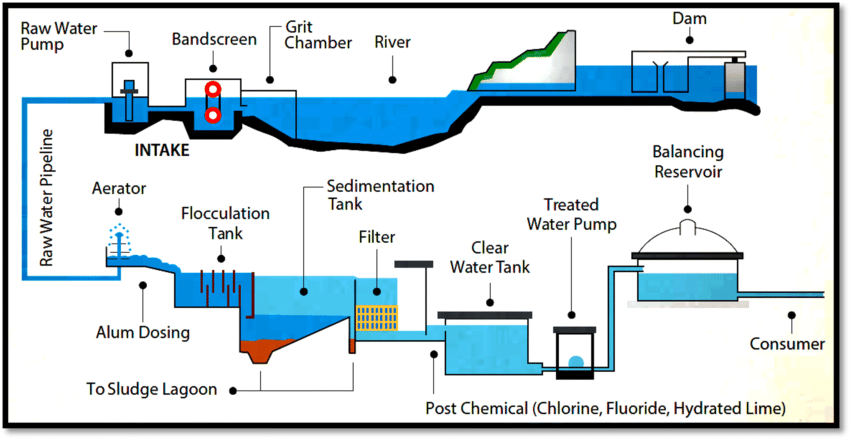
\includegraphics[scale=0.5]{WaterTreatment_9-01}
\caption{Conventional water treatment} \index{Conventional water treatment}
\end{center}
\end{figure}
\subsection{Source water treatment}\index{Source Water Treatment}
\begin{itemize}
\item Source water treatment in reservoirs or lakes includes treatment to contain algae growth.
\item Algal bloom is a sudden large increase in algae caused by weather or by nutrients. 
\item Reasons for controlling algae:
\begin{itemize}
\item Taste and odor problems
\item Shortened filter runs
\item Changes in pH - increases during the day, decreases at night
\item When algae dies, causes depletion of dissolved oxygen (DO)
\item Organic loading which is DBP pre-cursor resulting in TTHMs.
\end{itemize}
\item Algaecide such as blue stone, copper sulfate (CuSO$_4$) is used to control algae. 
\item Action level for copper is 1.3 mg/L·	·

\item Copper sulfate dose is usually specified in terms of pounds/acre. 
\item 5.4 lbs/acre is common dosage - the rate of application is based on the surface area of the reservoir not the volume
\item For water with alkalinify of higher than 150 mg/L, citric acid has to be mixed with CuSO$_4$ for it to be effective
\item Applying far more copper sulfate than necessary is uneconomical and ecologically undesirable. Excessive amounts of copper can kill fish and other bottom organisms, and copper tends to accumulate in bottom sediments. 
\end{itemize}
\subsection{Screening}\index{Screening}
\begin{itemize}
\item River water (the source of water used in our discussion) frequently contains suspended and floating debris varying in size from small rags to logs. Screening is usually the first major step where by large and suspended debris in the source water including sticks, leaves etc. is removed from the water before it enters the plant. 
\item Removing these solids is primarily to prevent damage to downstream equipment including pumps, prevent deposition of this debris in open channels or pipes, or in treatment processes.
\item The most important criteria used in the selection of a particular screening system for are the screen opening size and flow rate. Other important criteria include costs related to operation and equipment, plant hydraulics, debris handling requirements, and operator qualifications and availability. 
\item Depending on the characteristics of the source water, variety of screening devices including trash rakes, bar screens and wire mesh screens may be used. Very small screens can be used to screen out elements including algae in the water.
\item Typical screening devices used include:
\begin{itemize}
\item Trash Screens (Rakes) - used to remove rough or large debris.  The bar spacing in Rakes range from 1.5 to 4 inches.
\item Traveling Water Screens (Bandscreens) - these are placed in a channel of flowing water to remove floating or suspended debris.
\begin{figure}[h]
\begin{center}
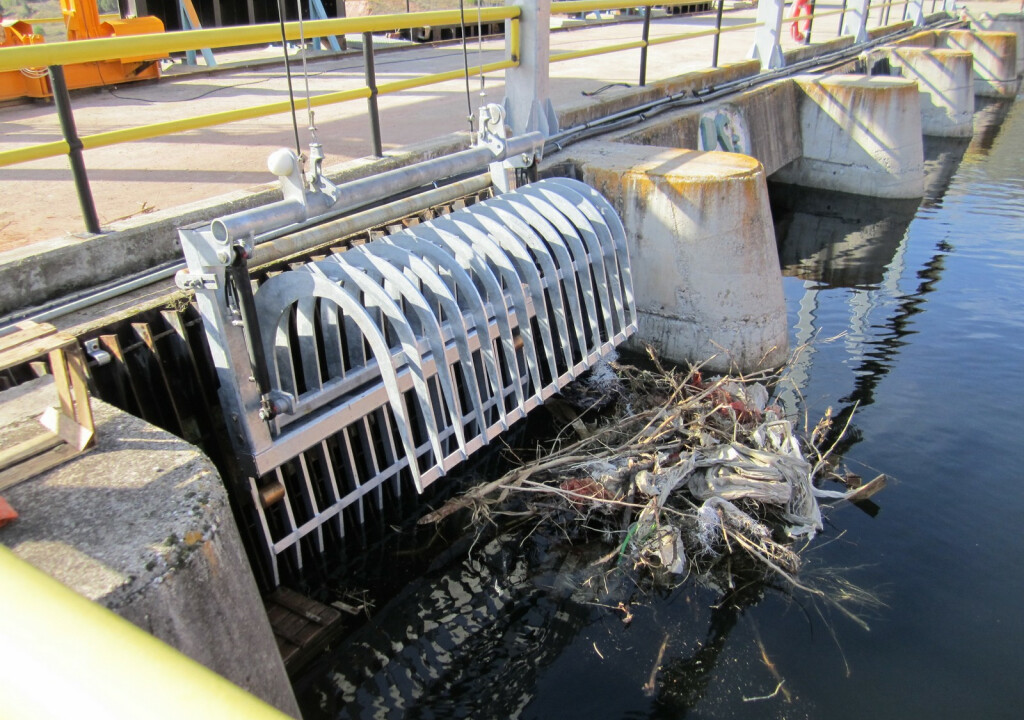
\includegraphics[scale=0.25]{TrashRakes}
\captionof{figure}{Trash rake}
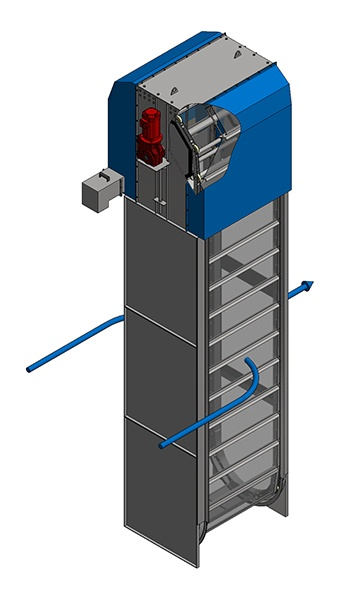
\includegraphics[scale=0.4]{TravellingScreen}
\captionof{figure}{Band screen}
\end{center}
\end{figure}
\end{itemize}

%\begin{center}
%\tcbox{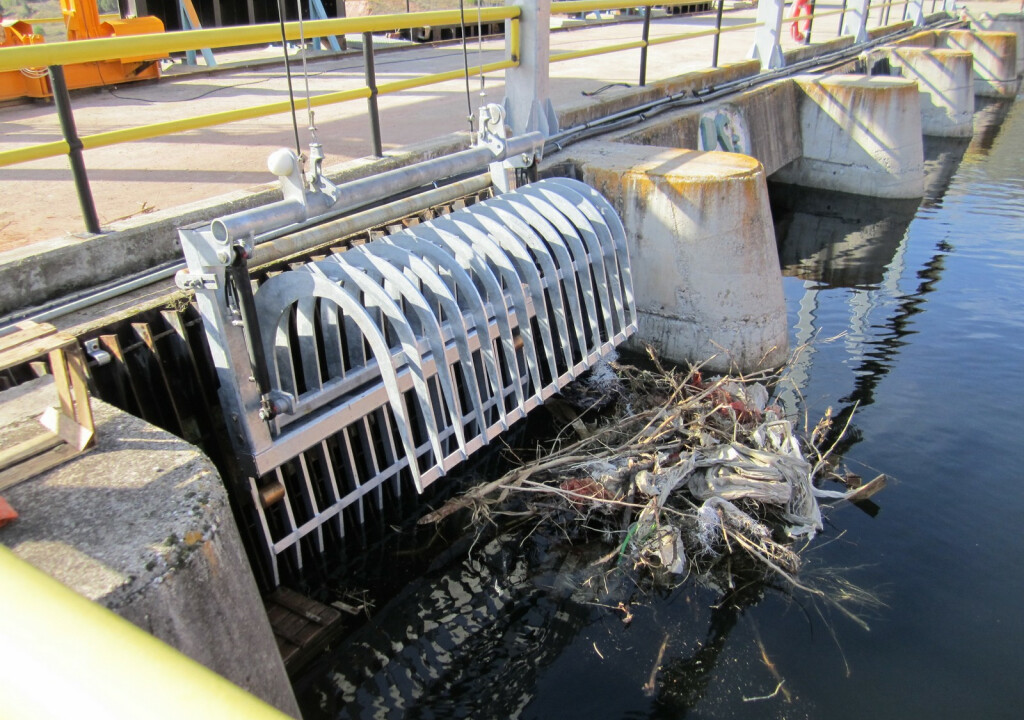
\includegraphics[width=6cm]{TrashRakes}}
%Trash Rakes
%\tcbox{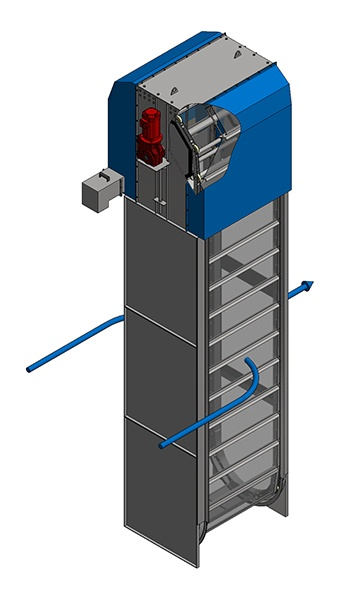
\includegraphics[width=6cm]{TravellingScreen}}
%\end{center}


\end{itemize}

\subsection{Coagulation and flocculation}\index{Coagulation and flocculation}
\begin{itemize}
\item A significant amount of suspended particles in the raw water are too small to be filtered or settled out in the sedimentation basin.  These particles, termed as colloids are non-settleable solids and include organic matter, silt, clay.
\item These particles impart turbidity and color to the water and may harbor pathogens and typically carry a negative electrostatic charge on its surface - negative \textbf{zeta potential}.  The like surface charge on these particles cause electrostatic repulsion (particles keep bouncing off one another) which makes these particles difficult to settle. 
\item Coagulation and flocculation are sequential processes both of which involve chemical addition.
\item For coagulation, either metal salt type coagulant - typically an aluminum salt such as alum or aluminum sulfate or an iron salt such as ferric or ferrous chloride or sulfate, polyaluminum chloride or a organic coagulant such as polyDADMAC or polyamine is used. The coagulant helps coalesce the non-settleable solids into larger particles.
\item Sodium aluminate is often used as an aide to alum coagulation particularly for cold water and during lime softening.
\item Coagulation is affected by changes in the water's pH, alkalinity, temperature, time, velocity and zeta potential.

\item The effectiveness of a coagulant is generally pH dependent. Water with a color will coagulate better at low pH (4.4-6) with alum.

\item Alkalinity is needed to provide anions, such as (OH$^-$) for forming insoluble compounds to precipitate them out. It could be naturally present in the water or needed to be added as hydroxides, carbonates, or bicarbonates.  Generally 1 part alum uses 0.5 parts alkalinity for proper coagulation.

\item The higher the temperature, the faster the reaction, and the more effective is the coagulation. Winter temperature will slow down the reaction rate

\item The coagulation process requires rapid mixing of the water upon the addition of the coagulant followed by a sufficient contact time prior to the flocculation step.
\item The flocculant which is added after the coagulation step is to make even larger, more compact and settleable - \textbf{floc}, from the coagulated solids.
\item Flocculants are typically long chain organic compounds - polymers with charged end groups.  \textbf{anionic polymers} have a negative end group whereas \textbf{nonionic polymers} have balanced - positive and negative end groups.
\item For the floc formed to remain intact, the polymer is gently "folded in" with the coagulated solids.  The flocculation is done in a flocculator which have a detention time of 5 -30 minutes and the water is mixed with the polymer using slow moving paddles.
\item Coagulant aids - chemicals which aid in the coagulation process and strengthening the flow include:
\begin{itemize}
\item Alakalinity enahncers - lime, Soda ash, caustic soda and sodium bicarbonate.
\item Weighting agents - calcimu carbonate and bentonite clay.  These are used in waters which are low in tubidity and high in color which under normal condition would have formed weak, slow settlling floc.
\item Activated sililca - sodium silicate activated by hypochlorous acid is often used as a coagulant aid with alum.
\end{itemize}


\end{itemize}

\item These will usually be used in conjunction with a primary coagulant such as ferric chloride, ferric sulfate, or alum.

\vspace{0.6cm}

\vspace{0.6cm}
\begin{figure}[H]
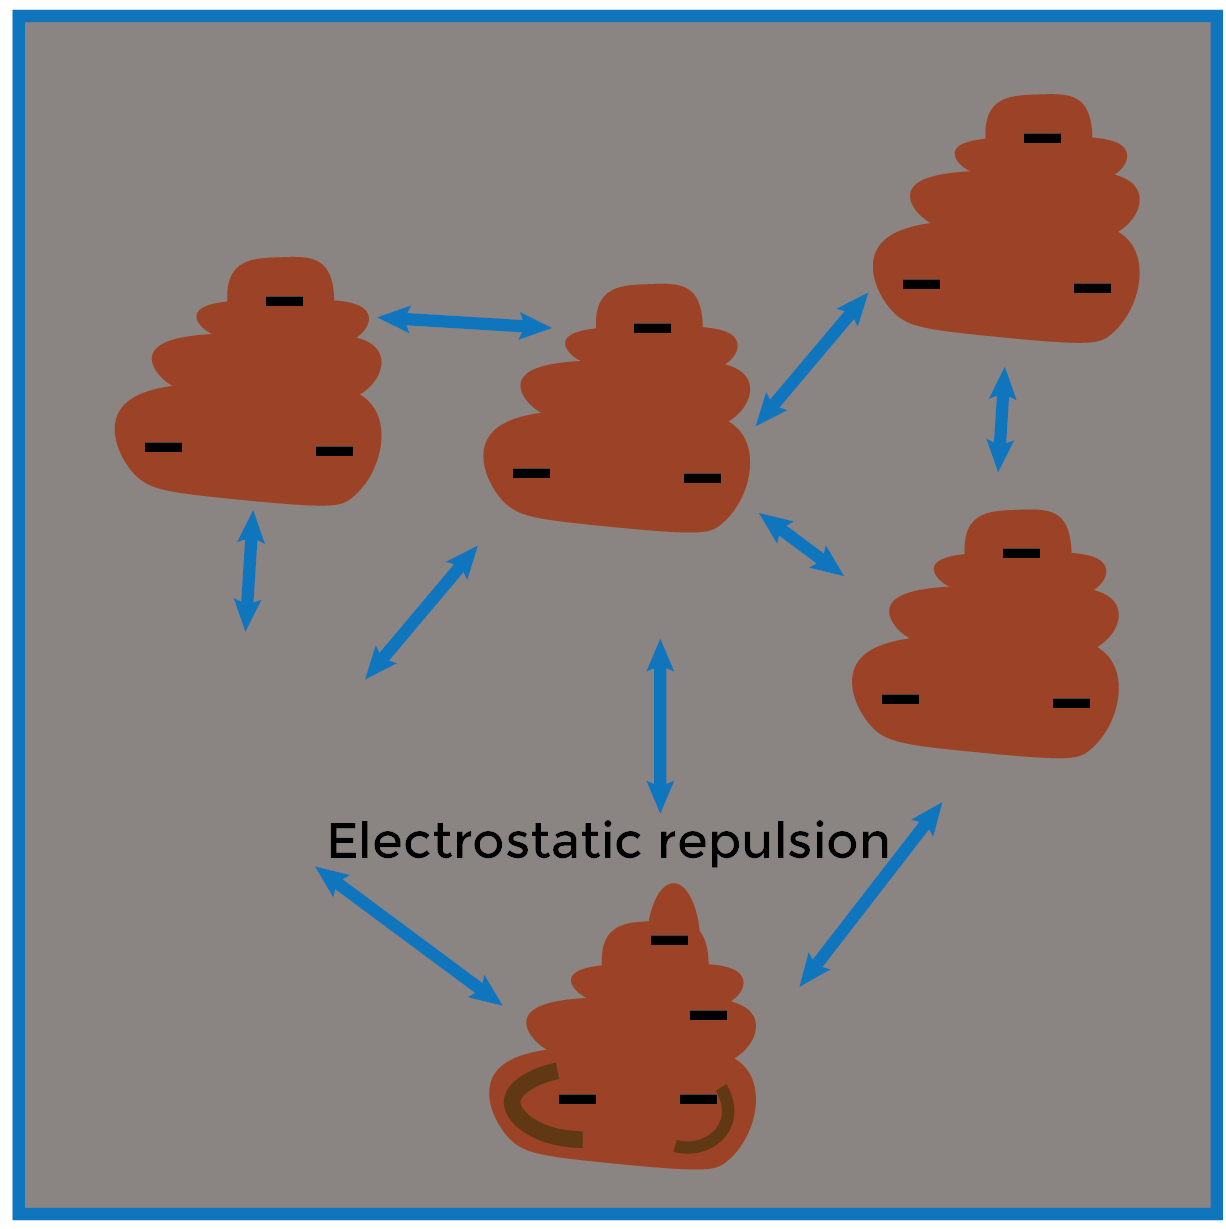
\includegraphics[scale=.13]{CEPTInitial} \hspace{0.7 cm}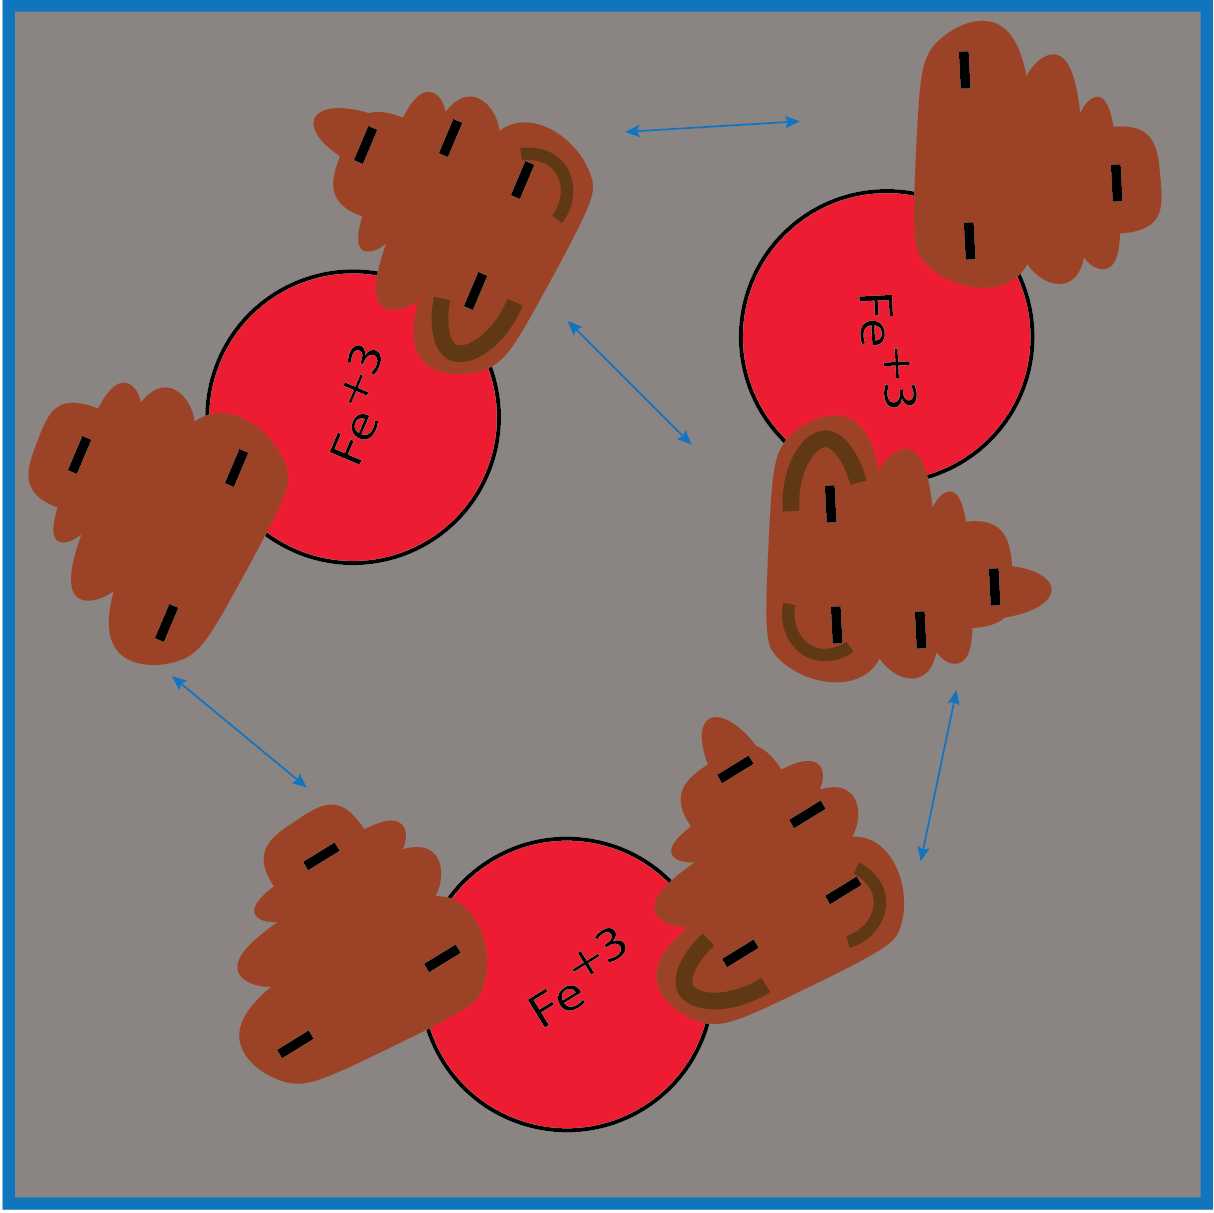
\includegraphics[scale=.13]{CEPTCoagulation}\hspace{0.7 cm}
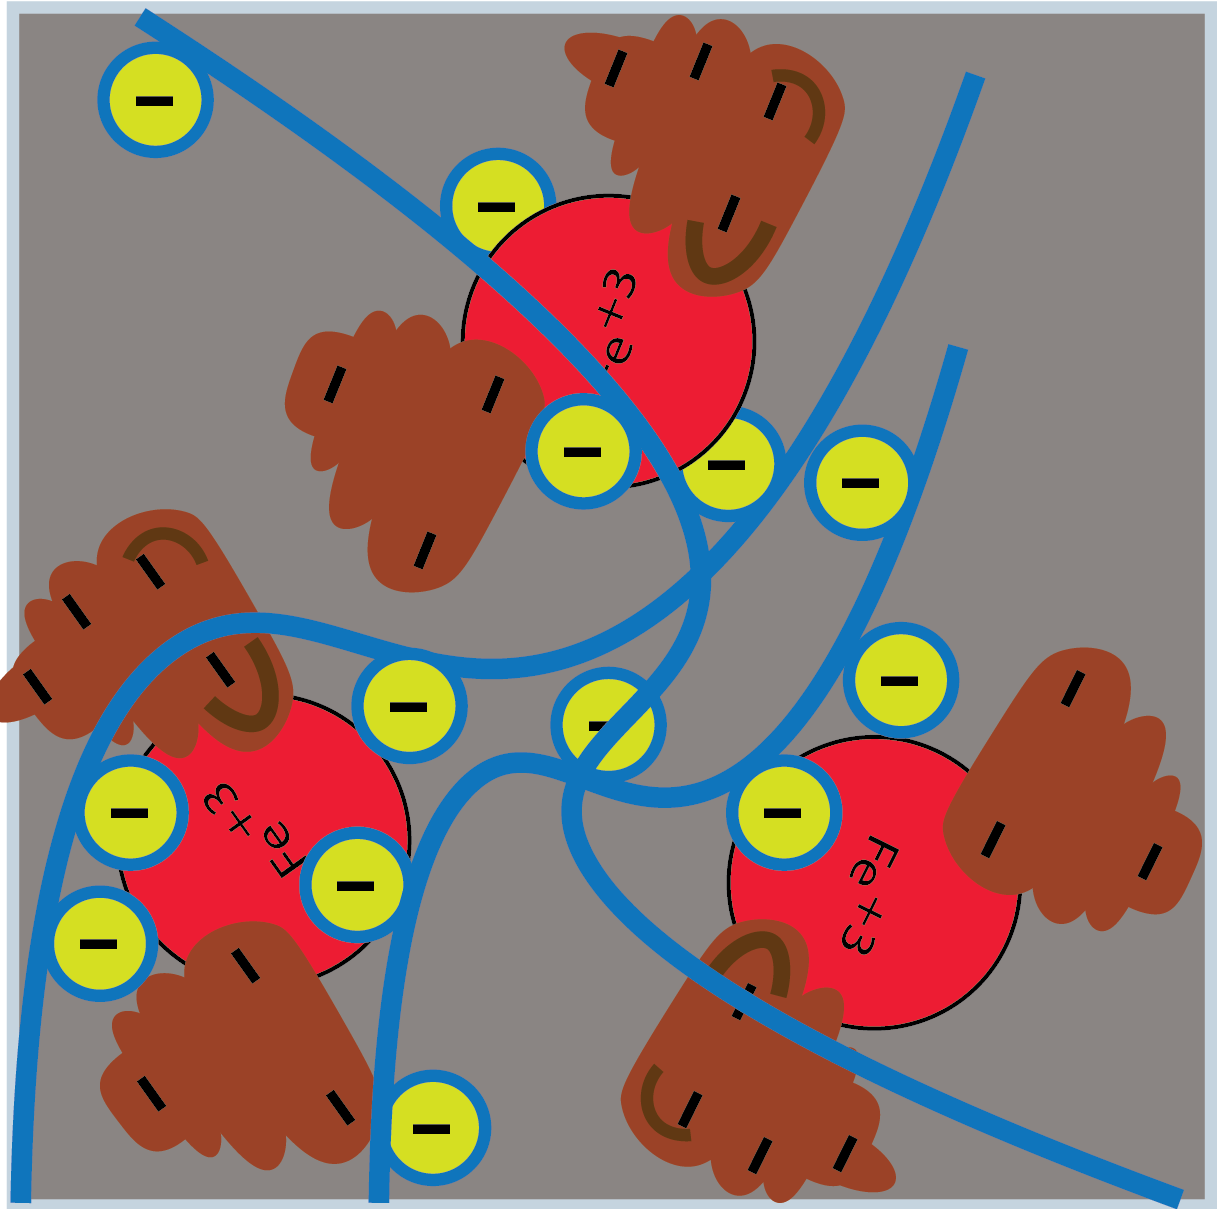
\includegraphics[scale=.13]{CEPTFlocculation}\\
\hspace{0.8cm} \textbf{Untreated Water}\hspace{2.4 cm}\textbf{Coagulation}\hspace{3 cm}\textbf{Flocculation}\\	
\caption{Coagulation-flocculation graphic}
\label{Coagulation-flocculation graphic}
\end{figure}

\item Determining the amount and type of coagulant used changes based on a variety of process conditions and quality of water. For example, a heavy rain will greatly impact the influent, or raw, water in a municipal treatment plant.

\item The jar test is a standard method in which various amounts of coagulant and flocculation times are tested on a raw water sample. There are multiple samples to test before implementation into a larger volume of the water treatment process.

\begin{figure}[h]
\begin{center}
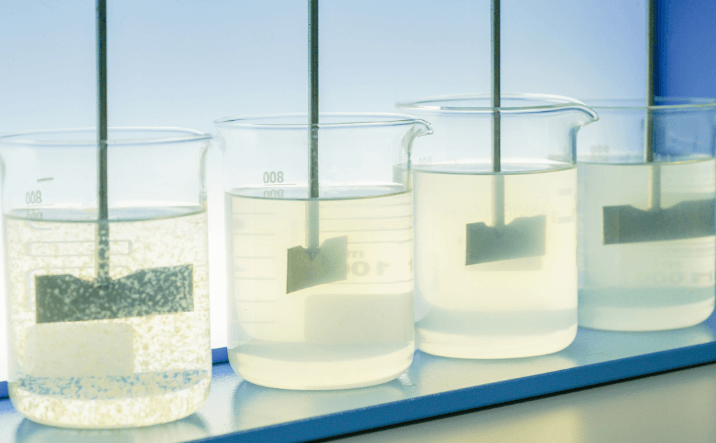
\includegraphics[scale=0.2]{JarTest}
\caption{Jar testing}
\label{table:Jartesting}
\end{center}
\end{figure}	

\end{itemize}
\subsection{Clarification/sedimentation}\index{Clarification/sedimentation}
\begin{itemize}
\item Clarification, or sedimentation, is the third step in conventional water treatment, after coagulation and flocculation and before filtration.
\item In the sedimentation basin the flocculated particles settle out under the influence of gravity.
\item In conventional sedimentation basins the solids drop out (settle) as the water slowly flows across the basin from the influent to effluent end.
\item Sedimentation basins are designed to create conditions in which the water flows very slowly through the basin, with minimal turbulence.
\item Conventional sedimentation basins are typically rectangular or cylindrical concrete or steel vessels which incorporate a horizontal flow of water.
\end{itemize}

			\begin{center}
				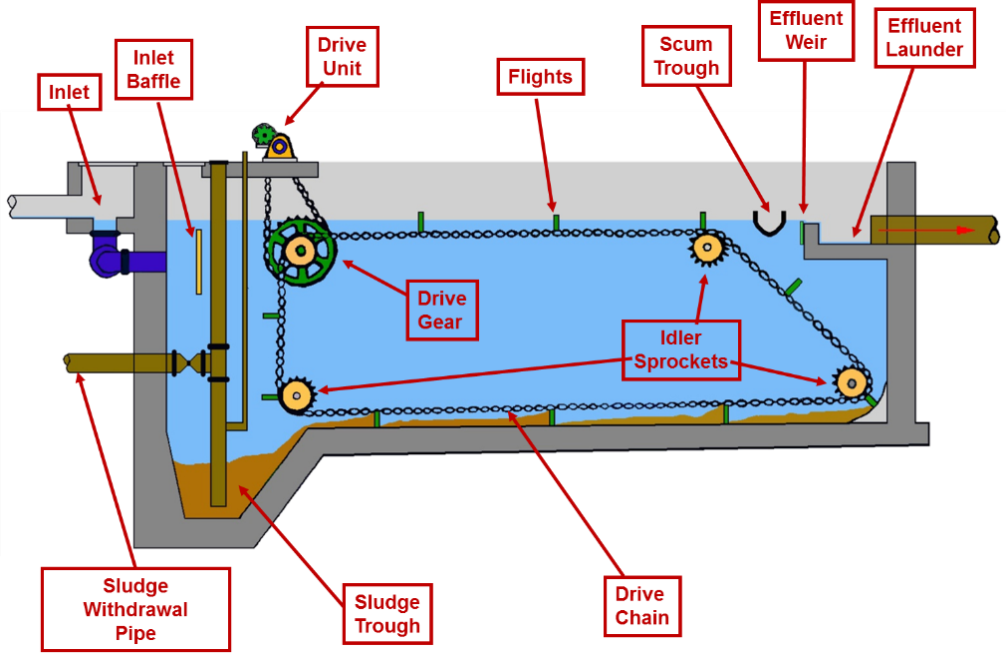
\includegraphics[scale=0.9]{RectangularClarifier}\\
				Cross section of a Rectangular Clarifier\\

				
\includegraphics[scale=0.1]{Blank}\\
				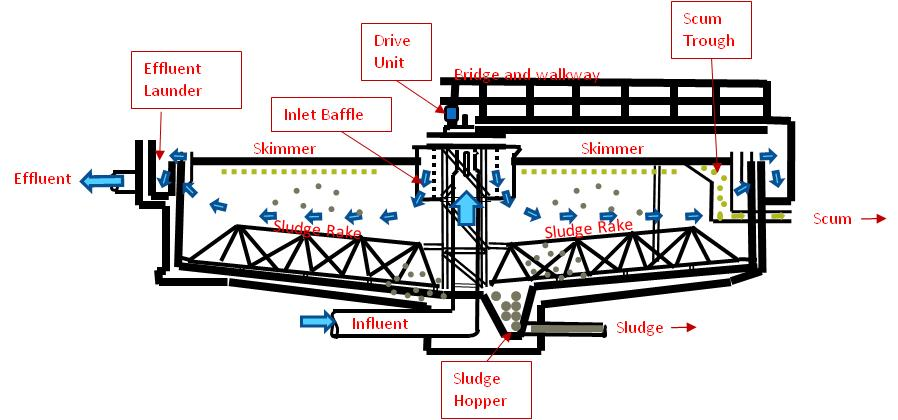
\includegraphics[scale=0.6]{CircularClarifierAI}\\
				Schematic cross section of a circular clarifier\\
				%
\includegraphics[scale=0.1]{Blank}\\
				%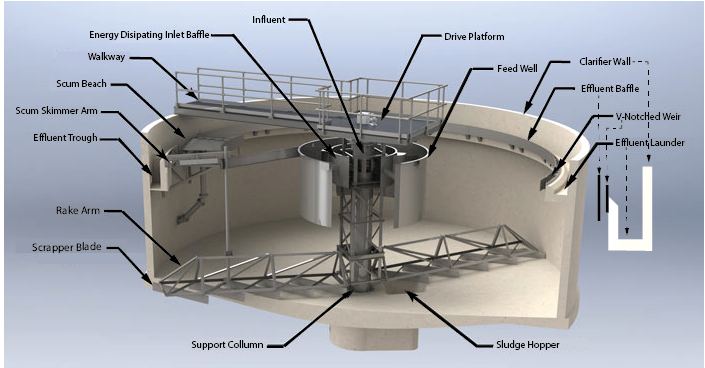
\includegraphics[scale=0.65]{CircularClarifier3}\\
				%Cross section of a circular clarifier\\
			\end{center}
				%
\includegraphics[scale=0.03]{Blank}\\


\subsubsection{Clarifier Zones}\index{Clarifier Zones}		
	\begin{itemize}
		\item Inlet Zone: is where the water enters the end of a rectangular tank, or the center of a circular or square tank. The Inlet Zone is designed to accomplish two objectives:
			\begin{enumerate}
				\item Reduce the velocity (dissipate 									energy in the incoming water).  This is accomplished by the inlet baffle.
				\item Distribute the flow evenly using baffles in front of the influent baffle.
			\end{enumerate}
				
		\item Settling Zone: This is the largest portion of the tank where the water is flowing very slowly allowing the solids to settle.  The clarifier is said to be short circuiting if 		the velocity of the water is greater in some sections than in others. The water passing through the higher velocity region will have a reduced detention time and settleable solids will carry through with this water as it exits the clarifier.
		\item Sludge Zone: Sludge zone is the bottom of the tank where the 	settled solids collect and compact. Sludge rakes push the sludge to one end or the center of the tank so that it can be pumped out. 
		\item Skimming Zone: The skimming zone is at the surface of the tank for removing scum removing
		lighter solids which float to the surface.  
		\item Outlet Zone: This is the part of the clarifier where the settled water leaves the clarifier.  A channel called the effluent launder collects the effluent flow and directs it to the clarifier effluent piping. Weirs are installed along the edge of the effluent launder channel to skim the water evenly off the surface of the tank. 
		\end{itemize}


\subsection{Filtration}\index{Filtration}
\subsubsection{Process Basics}\index{Process Basics}
\begin{itemize}
\item The SWTR requires the filtration of surface water and groundwater under the direct influence of surface water.
\item Filtration is the mechanical removal of turbidity particles by passing the water through a porous medium, which is either a granular bed or a membrane.
\item The process of filtration involves straining, settling, and adsorption.
\item Filtration does not remove dissolved solids and by itelf is not effective for the removal of bacteria.
\item In filtration, solids are removed physically by:
\begin{itemize}
\item Straining – trapping particles, and 
\item Adsorption.
\end{itemize}
\item The filtration based treatment process can be either:
\begin{enumerate}
\item Conventional - which is a four step treatment process that consists of the treatment steps of coagualation, flocculation, sedimentation and rapid sand filtration.  
\item Direct - where the sedimentation step is omitted. It is for areas with high quality of water and allows for cost and space savings by eliminating the need for sedimentation basins.  
\end{enumerate}
\begin{figure}[H]
\begin{center}
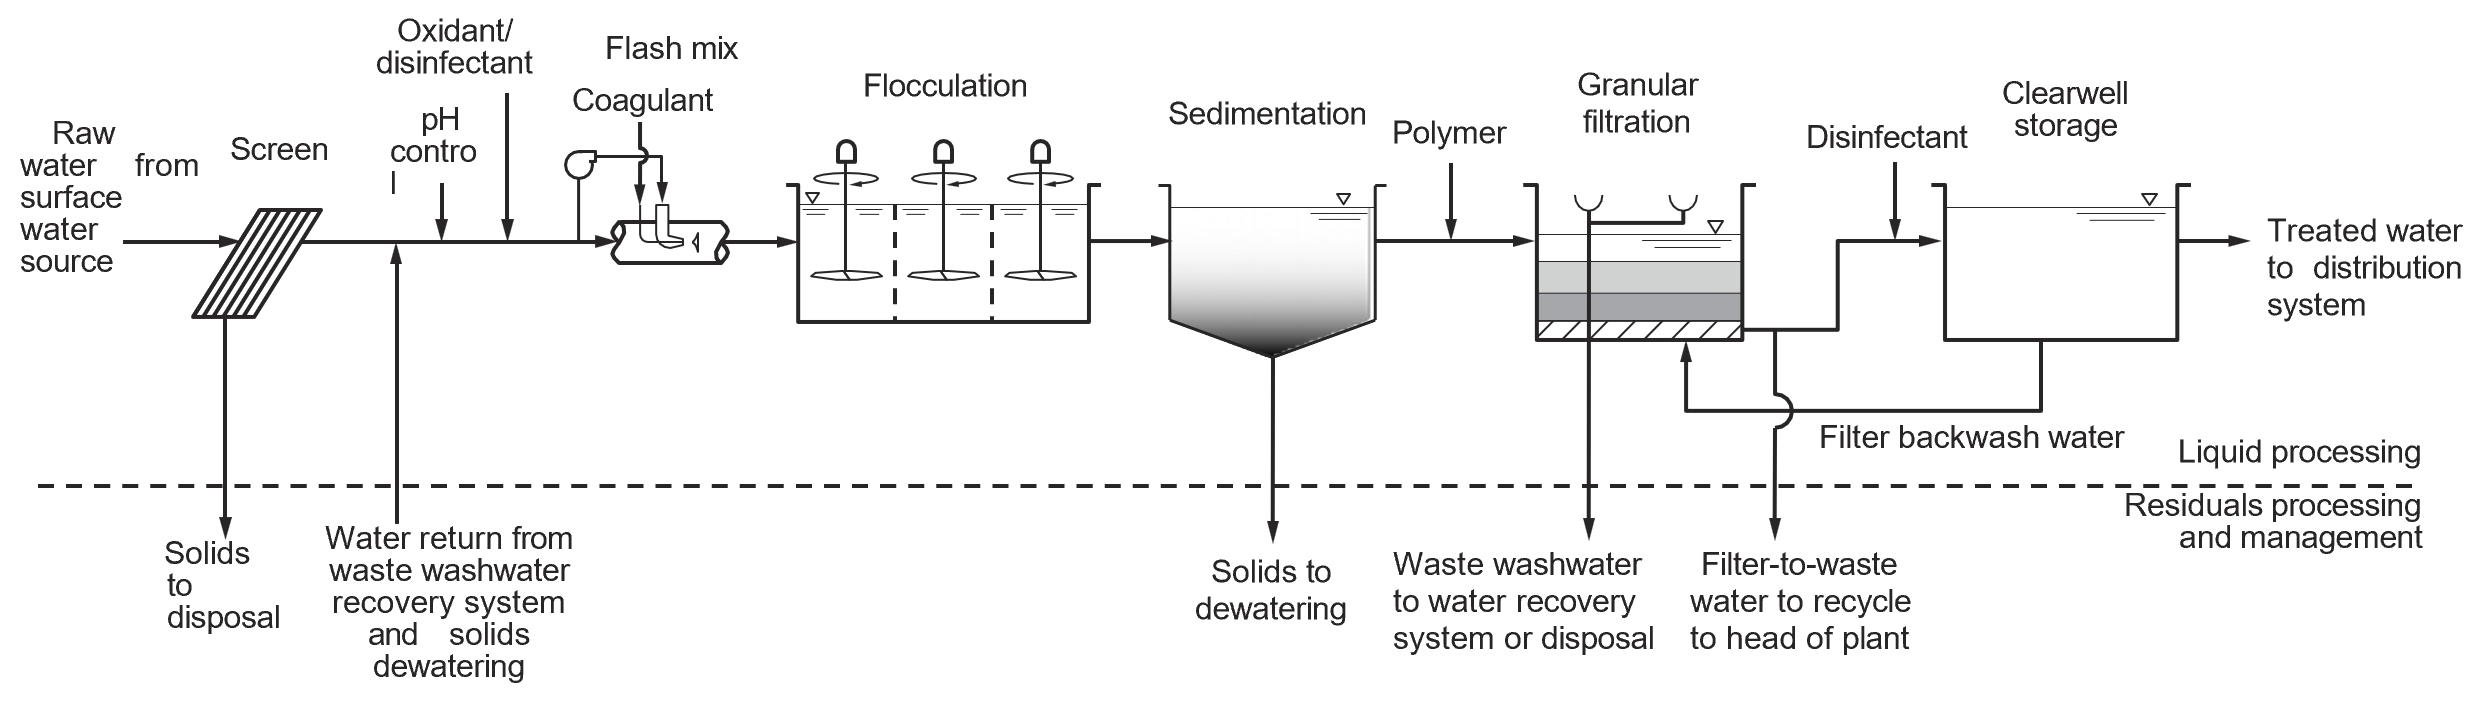
\includegraphics[scale=0.75]{ConventionalFiltration}\\
\captionof{figure}{Conventional filtration}%\caption{}
\label{Conventional filtration}
\end{center}
\end{figure}

\begin{figure}[H]
\begin{center}
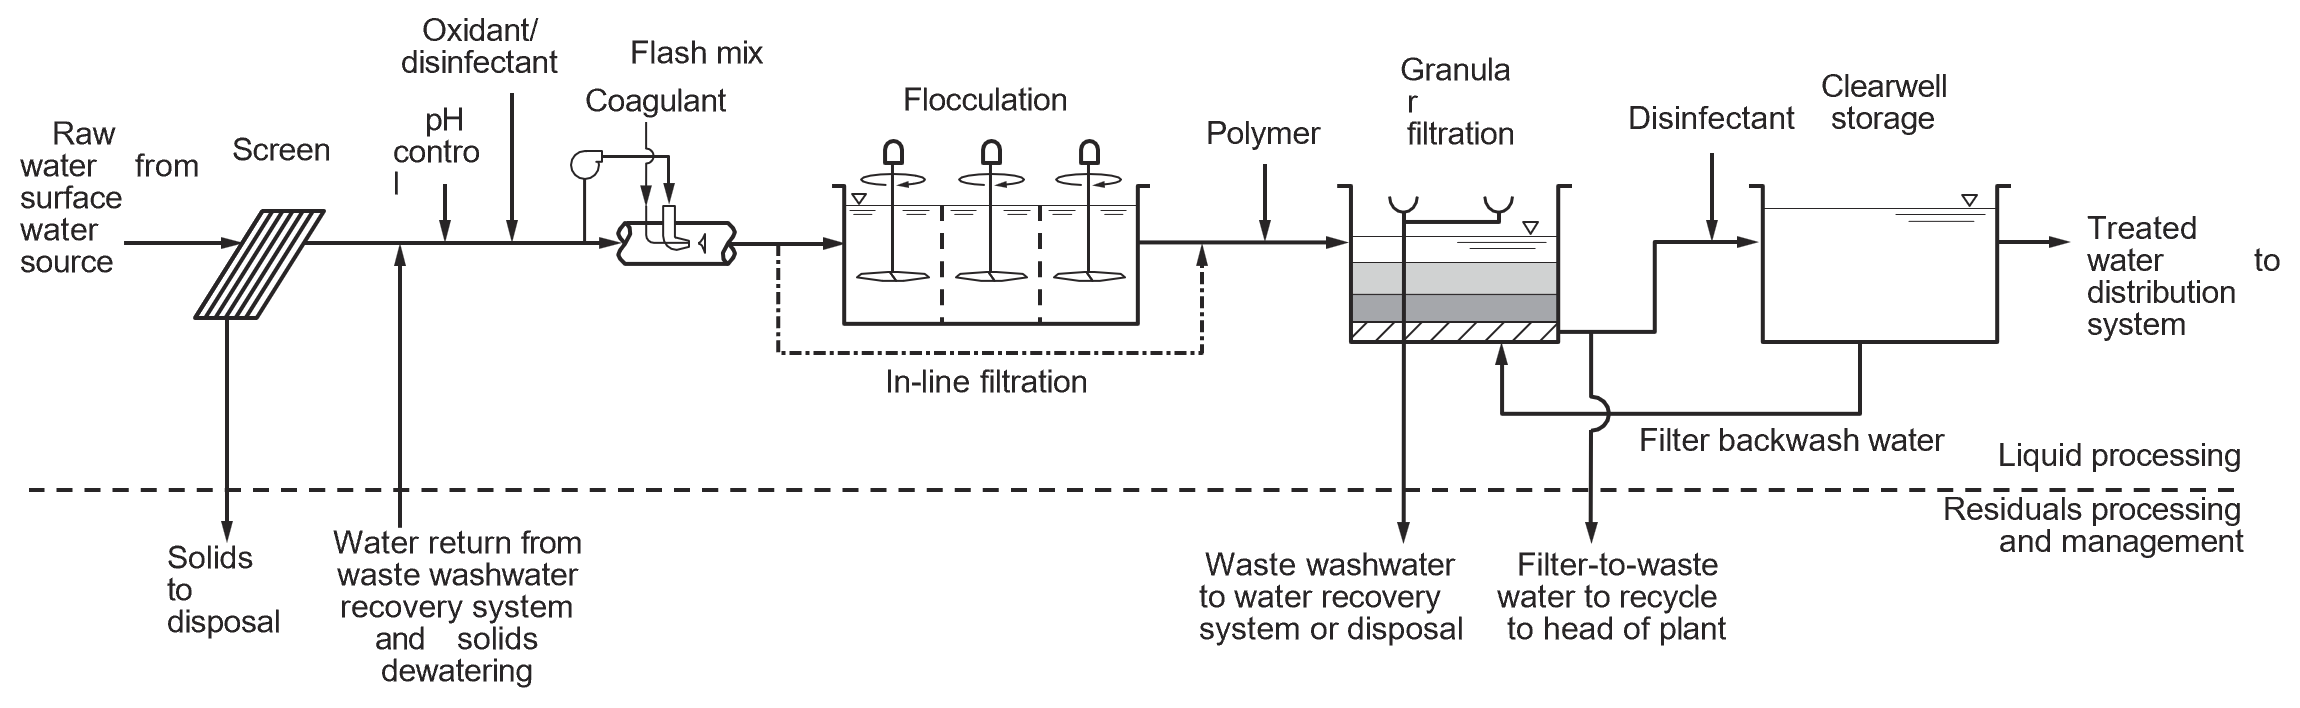
\includegraphics[scale=0.75]{DirectFiltration}\\
\captionof{figure}{Direct filtration}%\caption{}
\label{Direct filtration}
\end{center}
\end{figure}
\item Filters can also be classified as:
\begin{itemize}
\item Gravity – open to atmosphere and rely on the depth of water above the filter media to provide
the driving force to pass water through the media.
\item Pressure – utilize a pressure vessel to contain the media and can operate with a much higher driving force to pass water through the media.
\end{itemize}
\item Rapid gravity filters and slow sand filters are the two major types of filters used for water treatment.

\item Rapid filtration has following features that allow it to operate at higher water loading rates:
\begin{enumerate}
\item A filter bed of granular material that has been processed to a more uniform size than typically found in nature.
\item Use of a coagulant to precondition the water, and
\item Mechanical and hydraulic systems to efficiently remove collected solids from the bed.
\end{enumerate}
\item The rapid filtration
cycle consists of two stages: 
\begin{enumerate}
\item Filtration stage, when water flows downward through the filter bed and particles collect within the bed, and 
\item Backwash stage, water flows in the direction opposite to remove the particles that have collected in the filter bed. Efficient removal of collected solids is a key component of rapid filtration systems, so while the backwashing stage is very short compared to the filtration stage, it is a very important part of the filtration cycle.
\end{enumerate}

\item Rapid filtration is classified by the level of pretreatment, as presented in Figure ~\ref{figure:RapidFiltrationbyPretreatmentLevel}. The most important factors that determine the required level of pretreatment are the raw-water quality and the preference and resources of the operating utility.

\begin{figure}[H]
\begin{center}
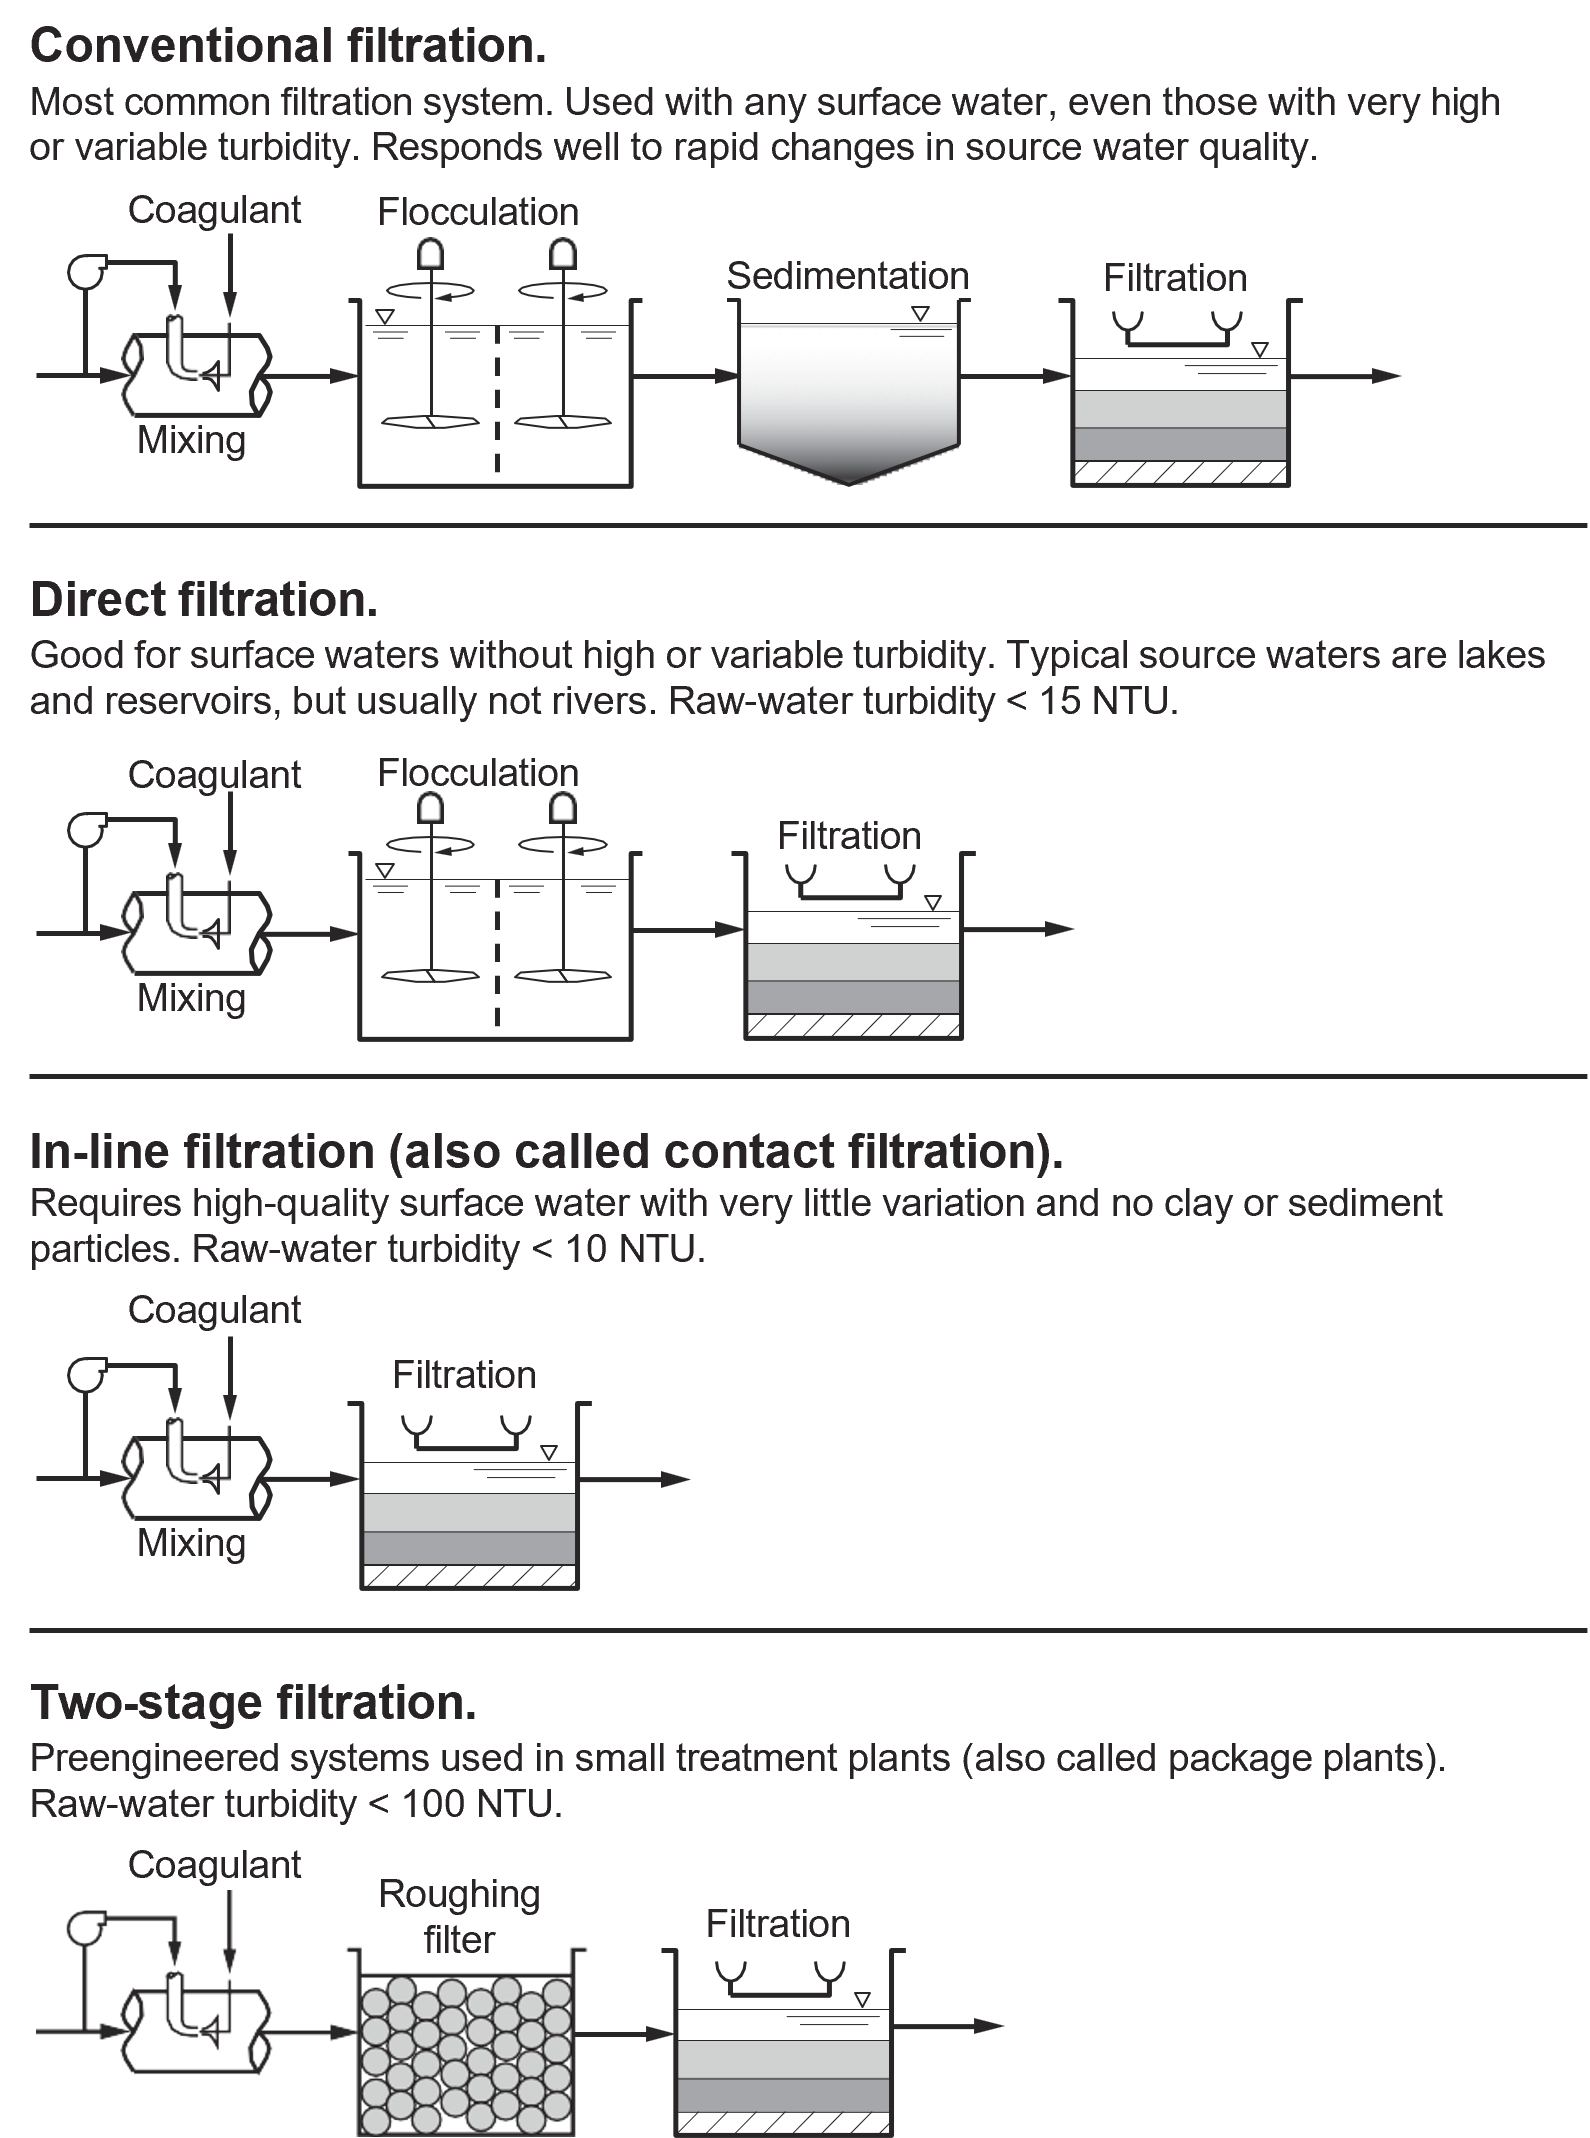
\includegraphics[scale=0.8]{RapidFiltrationbyPretreatmentLevel1}\\
%\captionof{figure}{Rapid Filtration by Pretreatment Level 0.8}%\caption{}
\end{center}

\caption{Rapid filtration by pretreatment level}  
                \label{figure:RapidFiltrationbyPretreatmentLevel} 
\end{figure}

\item In a slow sand filter there is a  layer - \textbf{Schmutzdecke} that develops on the top and is made up of microrganisms that feed on and break down organic material that is trapped on the surface of the filter. If the source water naturally contain low levels of nutrients, initial nutrient addition may be needed to develop this layer.

\item The Schmutzdecke enhances the particulate removal.  As the Schmutzdecke develops, the filter performance – as measured by the turbidity typically improves as the filter run progresses.

\item Filter media can consist of silica sand, greensand, anthracite coal, activated carbon,
and many other types of media. 
\item Filter media maybe a single media or mixed to provide improved filtration characteristics. 
\item Two most common types of granular media filters include dual-media filters such as anthracite coal and silica sand and tri-media which have anthracite coal, silica sand and fine garnet. 
\item Greensand media which incorporates potassium permanganate and manganese greensand which is the mineral called glauconite coated with manganese oxide.  Manganese greensand is a popular filtration media choice as it removes dissolved iron and manganese, hydrogen sulfide, radium and arsenic. Regeneration of traditional Greensand every six to twelve months with permanganate is recommended.
\item Activated carbon can be used as a topping for silica sand.  The activated carbon  does not only remove solids but also helps adsorb organic contaminants.
\item Pre-coat filters, utilize a slurry of raw water with diatomaceous earth (DE) as a pre-coat on a septum filter media which then captures the turbidity causing particles from raw water.  The filtration process is followed by a backwash cycle to remove the filtered cake buildup.  Precoat filtration is used to remove very small particulate matter, oil particles, and even bacteria from water. This method is practical only for relatively small quantities of water which contain low concentrations of contaminants.

\begin{figure}[H]
\begin{center}
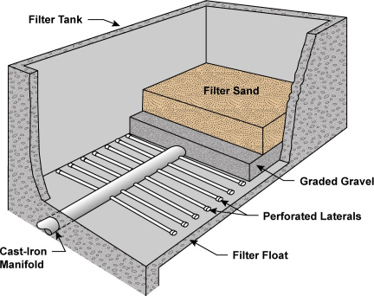
\includegraphics[scale=.6]{RapidSandFilter} \hspace{0.7 cm}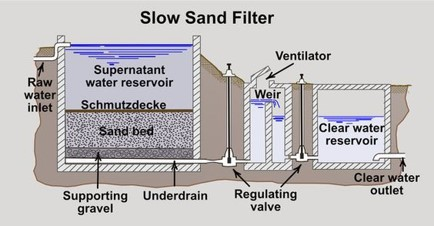
\includegraphics[scale=0.6]{SandFilter}\hspace{0.7 cm}\\
\textbf{Rapid Sand}\hspace{5 cm}\textbf{Slow Sand}\\
\vspace{0.8cm}
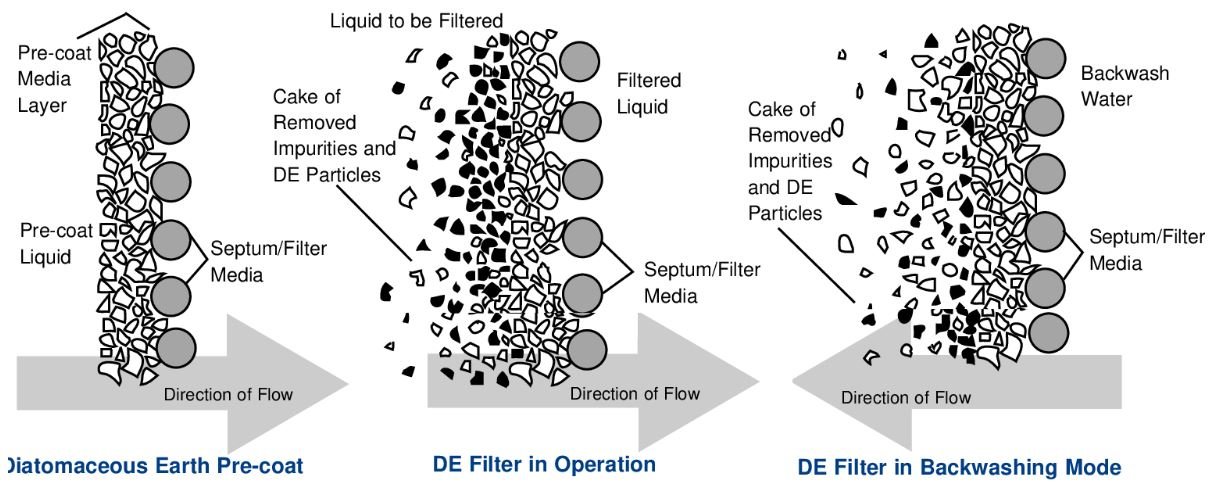
\includegraphics[scale=0.7]{DiatomaceousEarthFilter}\\
\textbf{Pre-coat - Diatomaceous Earth}\\
%\hspace{0.8cm} \textbf{Rapid Sand}\hspace{2.4 cm}\textbf{Slow Sand}\hspace{3 cm}\textbf{DE}\\	
\caption{Filter types}
\index{Filter types}
\end{center}
\end{figure}

\item Filters can also be classified as:
\begin{itemize}
\item Depth filtration – solids are removed within the granular material.  Example: Rapid granular bed filter
\item Cake filtration – solids are removed on the entering face of the granular material.  Example: Precoat
\end{itemize}
\item The Surface Water Treatment Rule describes five different types of filtration systems: 
\begin{itemize}
\item Conventional treatment
\item Direct filtration
\item Slow sand filtration
\item Diatomaceous earth filtration
\item Alternate filtration technologies such as bag filters and cartridge filters.
\end{itemize}
\item Besides using a filter media, process akin to filtration can also be accomplished using membranes. 
\item A membrane is a thin layer of material that will only allow certain compounds to pass through it. 
\item During operation, permeable components pass through the membrane and impermeable components are retained on the feed side. As a result, the product stream is relatively free of impermeable constituents and the waste stream is concentrated in impermeable constituents.
\item Which material will pass through the membrane is determined by the size and the chemical characteristics of the membrane and the material being filtered.
\item Membranes can be classified into two distinct physicochemical
processes: 
\begin{enumerate}
\item Membrane filtration which encompasses the use of:
\begin{enumerate}
\item Microfiltration (MF)membrane which function like a sieve. MF membrane pore size ranges from 0.1 to 1 micrometer ($\mu$m); therefore, they remove all particles bigger than 1 $\mu$m, including Cryptosporidium oocysts, Giardia cysts and all bacteria., and 
\item Ultrafiltration (UF) membranes which are similar to the microfiltration membranes except the pore size is smaller - 0.003 to 0.1 $\mu$m which removes very small particles including viruses and THM formation precursors.
\item Nanofiltration (NF) membranes which have nanometer (0.001 $\mu$m, or 1 nm) pore size and can remove all the particles above nanometer size - besides removing viruses, cysts, and bacteria they remove some dissolved substances including divalent ions such as Ca$^{+2}$ and Mg$^{+2}$,and are used for softening water and to reduce the concentration of organic matter to control disinfection by-product (DBP) formation.
\end{enumerate}
\item Reverse Osmosis (RO) where preferential diffusion of water through a semipermeable membrane in response to a concentration gradient.  
\begin{itemize}
\item In RO, the feed stream is a solution, or single-phase system, in which the constituents targeted for removal are truly dissolved solutes - ions such as sodium, chloride and dissolved NOM.
\item RO membranes are semipermeable - they function as sieves and selective diffusion membranes due to osmosis, allowing for specific dissolved substances to pass through. 
\item Osmosis is the passage of water through a semipermeable membrane from the lower concentration of the dissolved substances to the higher concentration to equalize the concentration on both sides of the membrane. The force with which water flows through the membrane is called osmotic pressure. The greater the difference in concentration on two sides of the membrane, the higher the osmotic pressure, and faster is the flow. In reverse osmosis, a pressure higher than the osmotic pressure is applied on the higher concentration side to force the water through the membrane in the reverse order. 
\item RO membranes  are used to treat seawater that has total dissolved solids (TDS) in the range of 3.5\% (35,000 mg/L) and other brackish water (TDS up to 3\%).  
\item RO is also capable of removing specific dissolved contaminants - pesticides, arsenic, nitrate, radionuclides.
\end{itemize}
\end{enumerate}

\begin{figure}[H]
\begin{center}
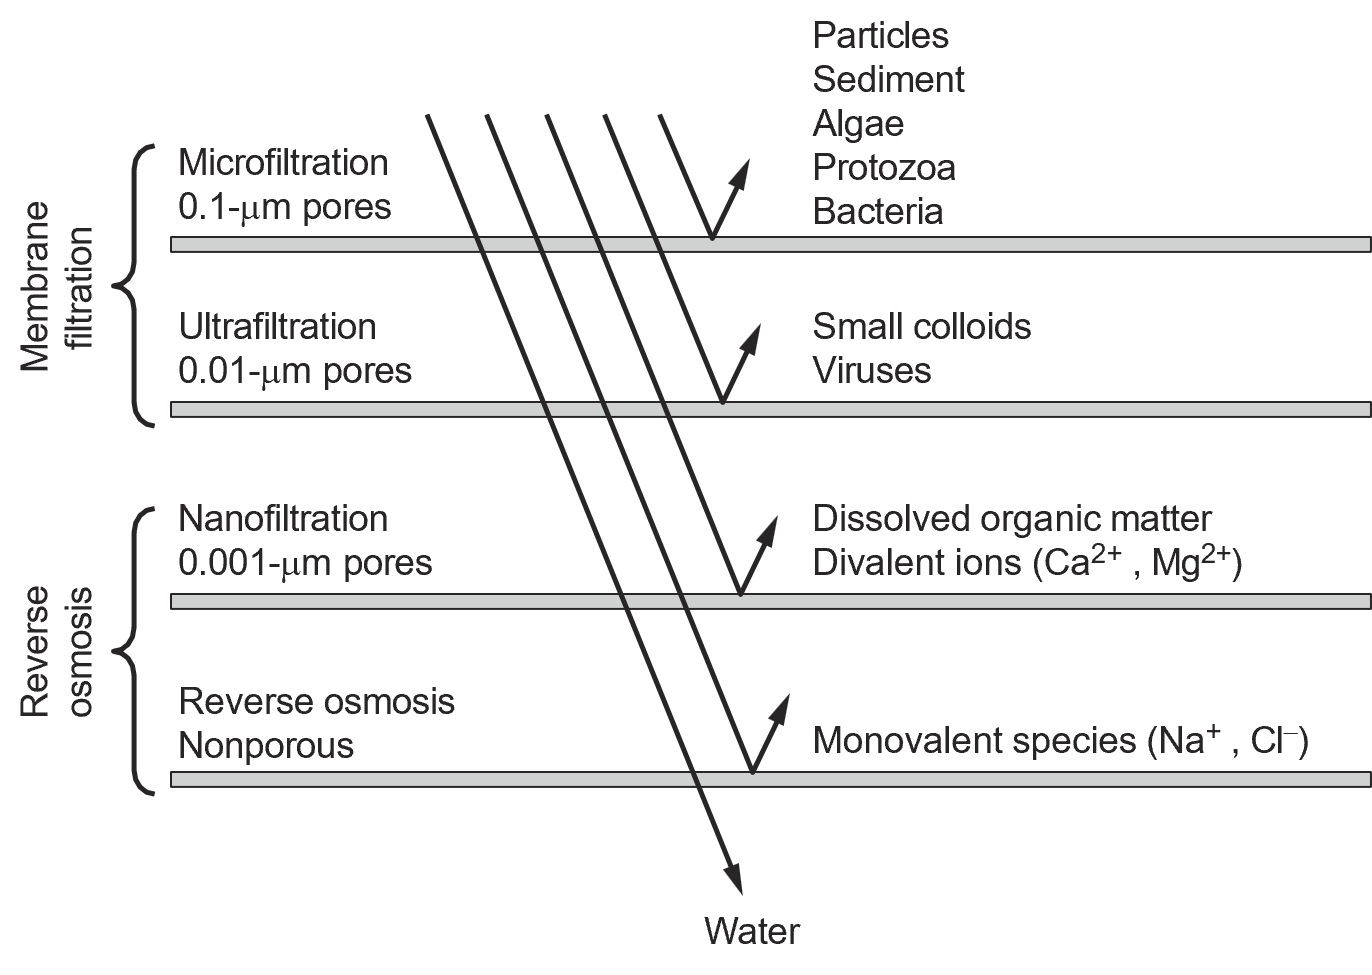
\includegraphics[scale=0.8]{MembraneProcesses}\\
\captionof{figure}{Membrane processes}%\caption{}
\label{Membrane processes}
\end{center}
\end{figure}
%\item Filter media in a rapid sand filter refers to the granular material used to remove particles from the filter influent. 
%\item Typical filter media in a rapid sand filter include sand (of course), and sometimes a “cap” of coal or granular activated carbon (GAC) placed on top of the sand media layer. 
%\item Filters with a sand and coal/carbon cap are referred to as dual media filters. Some rapid sand filters also contain a thin layer of garnet sand. This layer also tends to improve filter performance.  
%\item Filters with a layer of garnet sand are referred to as mixed media filters.
%\item Rapid sand filtration is the most common type of filtration used in water treatment. 
%\item Slow sand filtration is usually a feasible alternative for SWTR compliance only for small water systems with relatively high quality source water.
%\item Also, pre-treatment (example: coagulation/flocculation) and final disinfection are therefore needed. 
%
%
%
%\item Granular Bed and Pre-coat Filters are typically used for surface water treatment
%
%\item Media in Granular Bed filter is comprised of one or a combination of the following:
%\begin{itemize}
%\item Sand
%\item Anthracite
%\item Granular activated carbon
%\end{itemize}
%\item Pre-coat filters use a thin layer of very fine medium such as diatomaceous earth.  Precoat filtration is used to remove very small particulate matter, oil particles, and even bacteria from water. This method is practical only for relatively small quantities of water which contain low concentrations of contaminants.
%
%\item Gravity filters can be operated at different hydraulic rates
%\begin{itemize}
%\item Slow filters
%\item Rapid filters
%\end{itemize}
%


\end{itemize}
%\subsection{Conventional Treatment} \index{Conventional Treatment}
%
%\subsection{Direct Filtration} \index{Direct Filtration}
%
%\subsection{Slow Sand Filtration} \index{Slow Sand Filtration}
%
%Microfiltration membranes function like a sieve. There pore size ranges from 0.1 to 1 micrometer ($\mu$m); therefore, they remove all particles biggerthan 1 $\mu$m, including Cryptosporidium oocysts, Giardia cysts and all bacteria. They are successfully used for water treatment plants with less than12 million gallons per day capacity and low raw water turbidity.
%Ultrafiltration
%Ultrafiltration membranes are similar to the microfiltration membranes except the pore size is 0.003 to 0.1 $\mu$m to remove very small particles. Theyremove all particles bigger than this pore size, including viruses and THM formation precursors. They remove cysts and other pathogens by sixlogs, meaning 99.9999 percent removal. They are more expensive due to the smaller pore size. The finer the pore size, the more effective themembrane, and the more expensive it is.
%Nanofiltration
%Nanofiltration membranes have nanometer (0.001 $\mu$m, or 1 nm) pore size.  They remove all the particles above nanometer size. Besides removingviruses, cysts, and bacteria, they remove some dissolved substances.
%
%Reverse Osmosis
%Reverse osmosis membranes are semipermeable. They function as sieves and selective diffusion membranes due to osmosis, which allows some specific dissolved substances to pass through. Osmosis is the passage of water through a semipermeable membrane from the lower concentration of the dissolved substances to the higher concentration to equalize the concentration on both sides of the membrane. The force with which waterflows through the membrane is called osmotic pressure. The greater the difference in concentration on two sides of the membrane, the higher theosmotic pressure, and faster is the flow. In reverse osmosis, a pressure higher than the osmotic pressure is applied on the higher concentration sideto force the water through the membrane in the reverse order. These membranes will remove all the suspended particles larger than the pore sizeand only selective dissolved substances. These membranes remove substances like sodium, calcium, magnesium, and other metal compounds.They are used to treat seawater that has total dissolved solids (TDS) in the range of 3.5% (35,000 mg/L) and other brackish water (TDS up to 3%).
%
%
%
%
%
%There are common variations of the conventional treatment and direct filtration pro- cesses that can be used to meet regulatory water treatment goals, to improve process efficiency, and to reduce the operational complexity of surface water treatment pro- cesses. These include two-stage filtration and pressure filtration.
%
%
%
%\subsection{Rapid Sand Filters} \index{Rapid Sand Filters}
%
%
%\begin{figure}[H]
%\begin{center}
%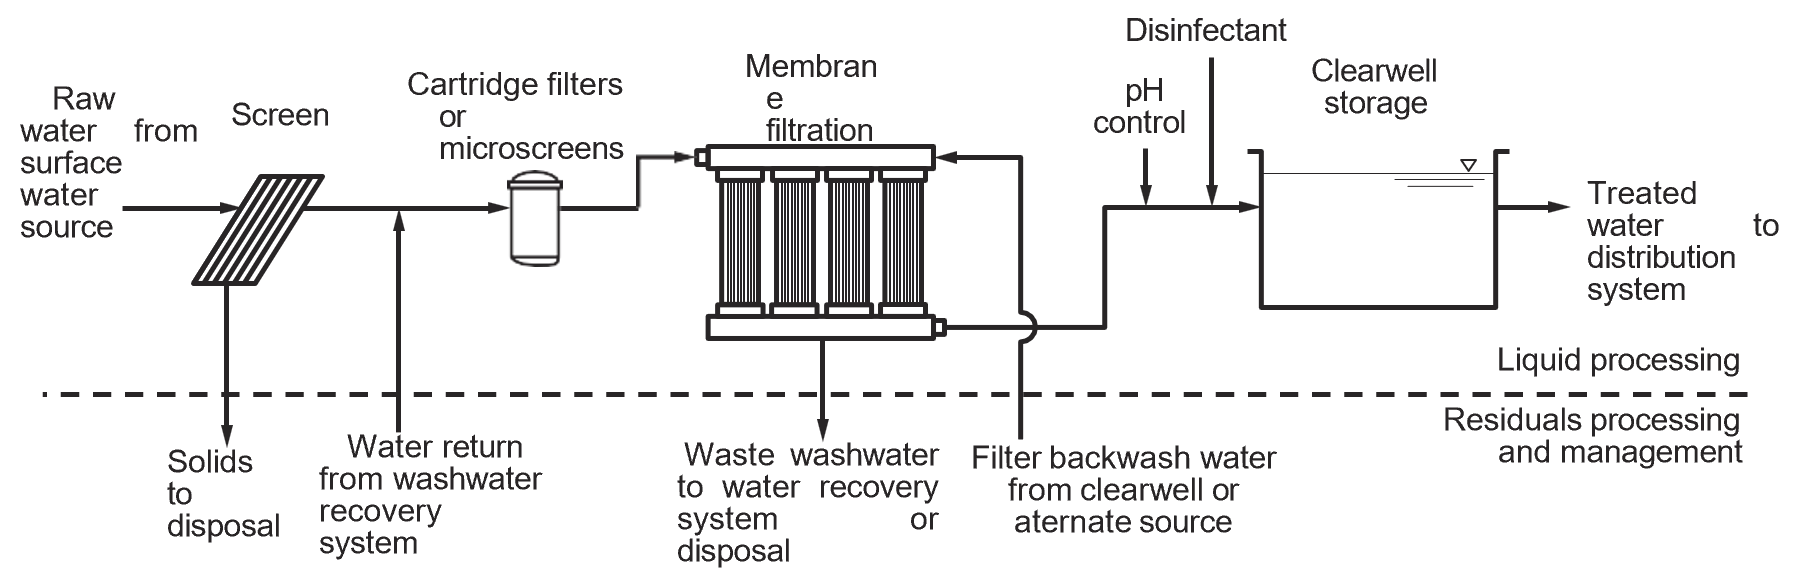
\includegraphics[scale=0.8]{MembraneFiltration}\\
%\captionof{figure}{Membrane Filtration 0.8}%\caption{}
%\end{center}
%\end{figure}
%
%\begin{figure}[H]
%\begin{center}
%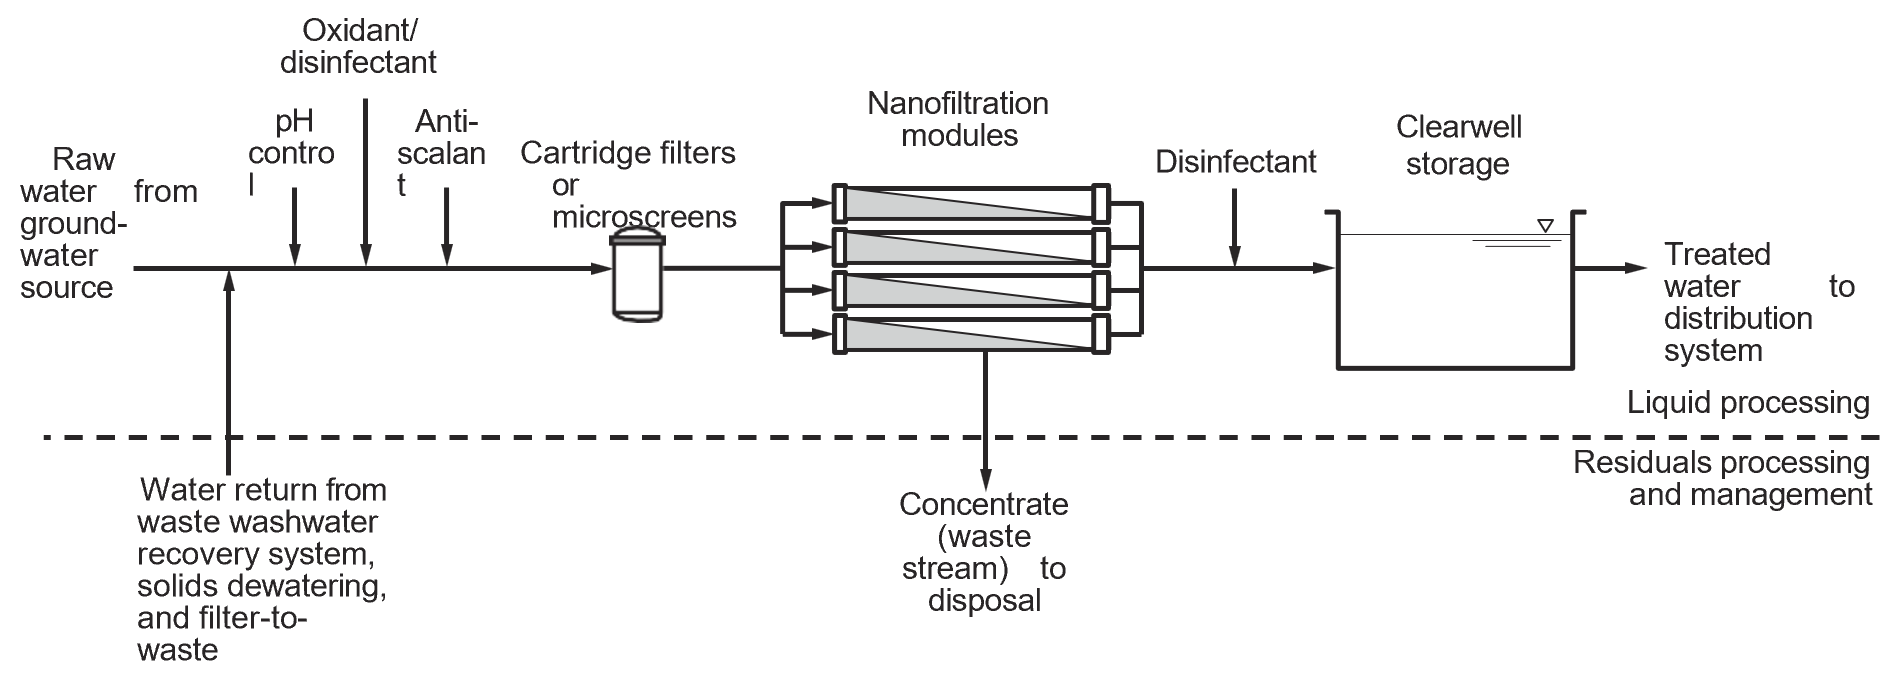
\includegraphics[scale=0.8]{NanoFilteringSoftening}\\
%\captionof{figure}{Nano Filtering Softening 0.8}%\caption{}
%\end{center}
%\end{figure}
%
%\begin{figure}[H]
%\begin{center}
%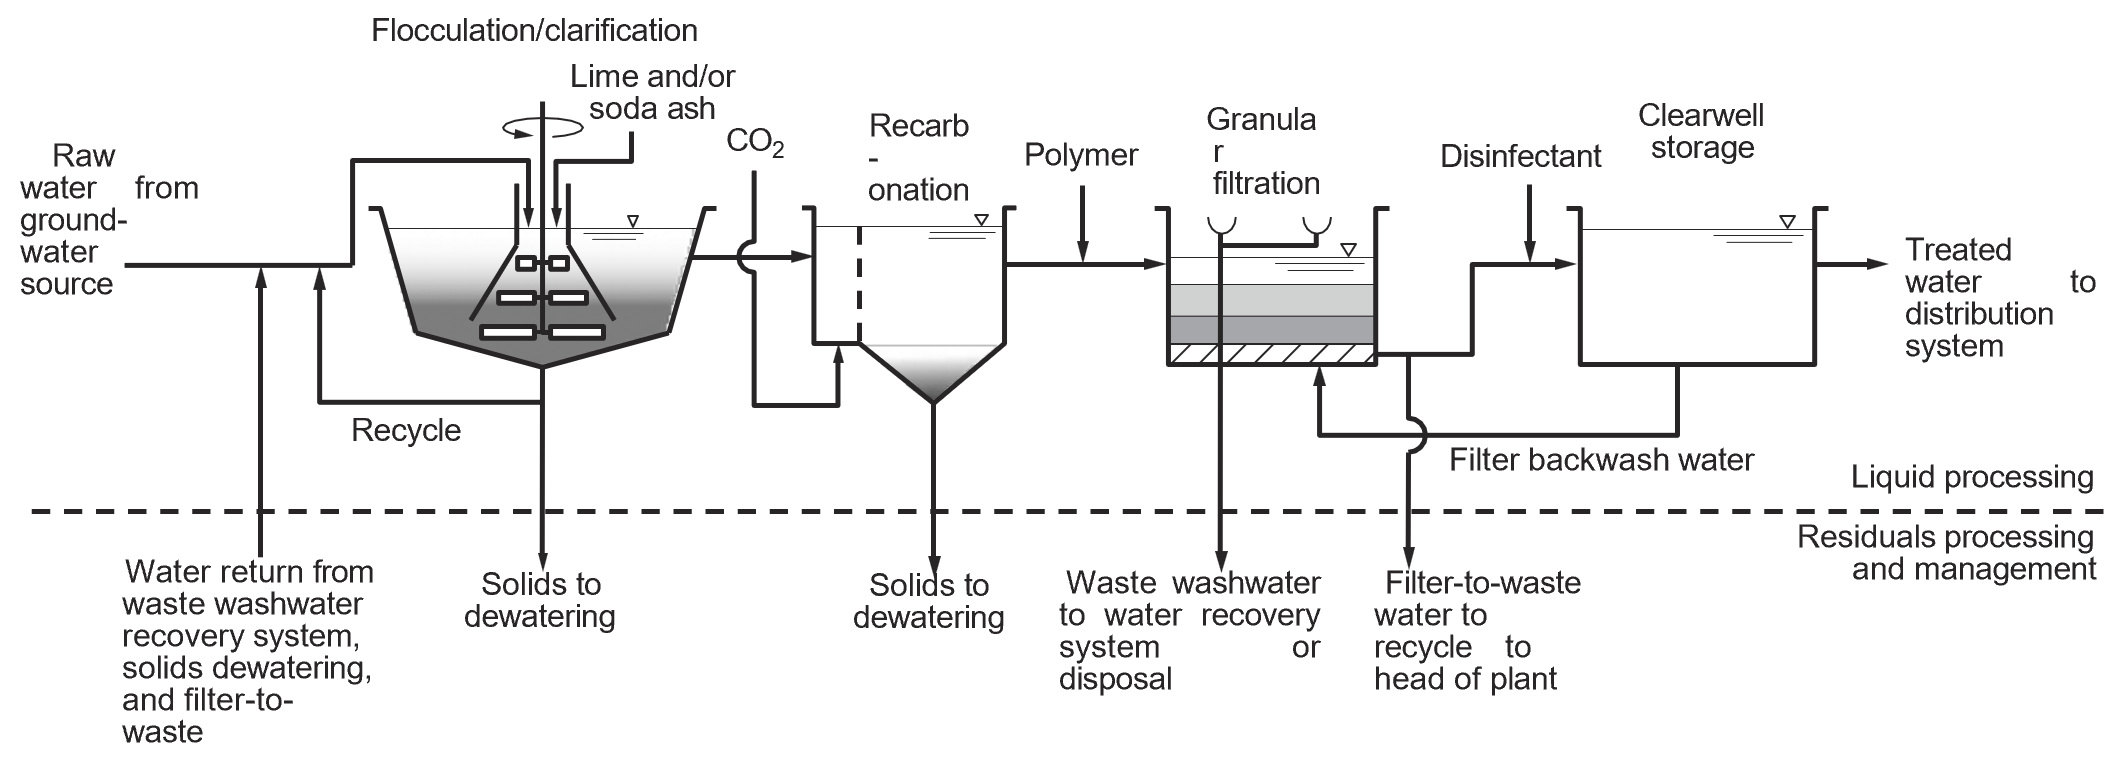
\includegraphics[scale=0.8]{SofteningLimeSoda}\\
%\captionof{figure}{Softening Lime-Soda 0.8}%\caption{}
%\end{center}
%\end{figure}
%
%\begin{figure}[H]
%\begin{center}
%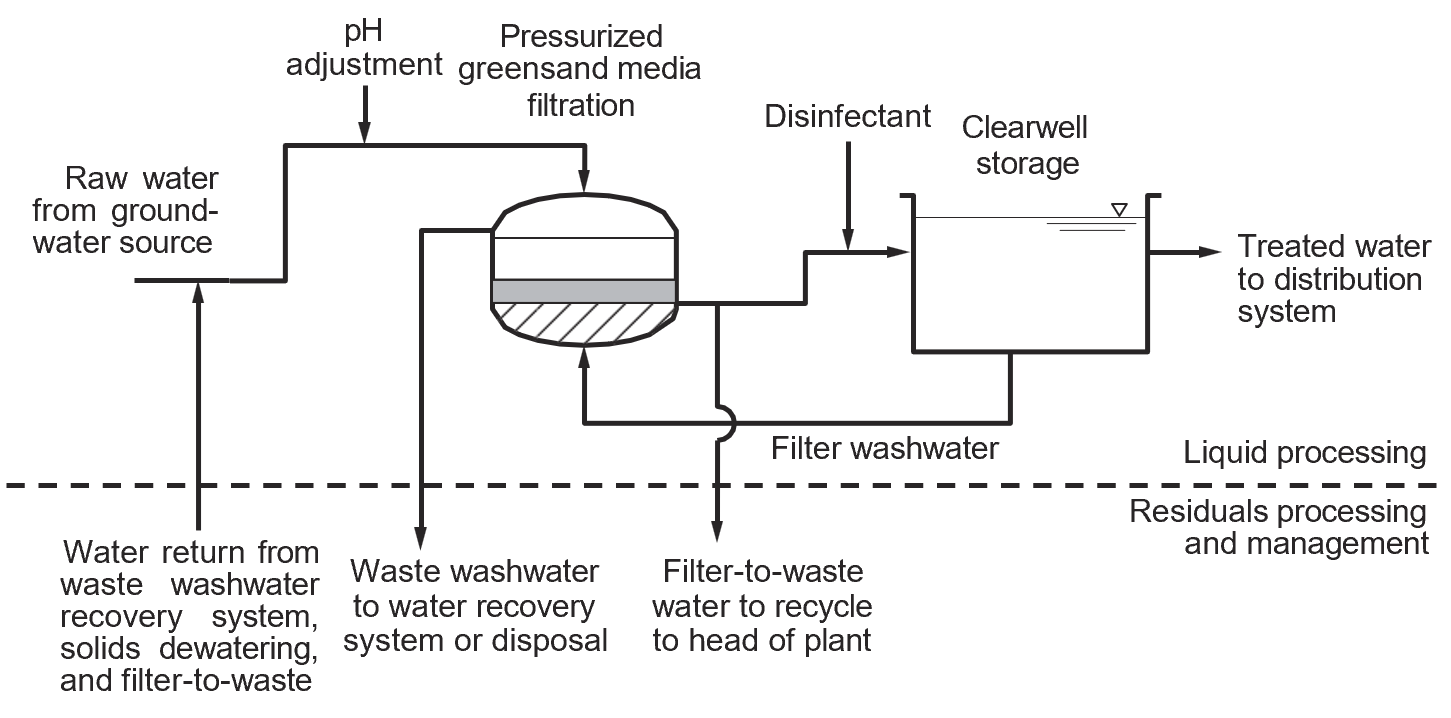
\includegraphics[scale=0.8]{FeMnRemovalGroundwater}\\
%\captionof{figure}{FeMnRemovalGroundwater 0.8}%\caption{}
%\end{center}
%\end{figure}
%
%\begin{figure}[H]
%\begin{center}
%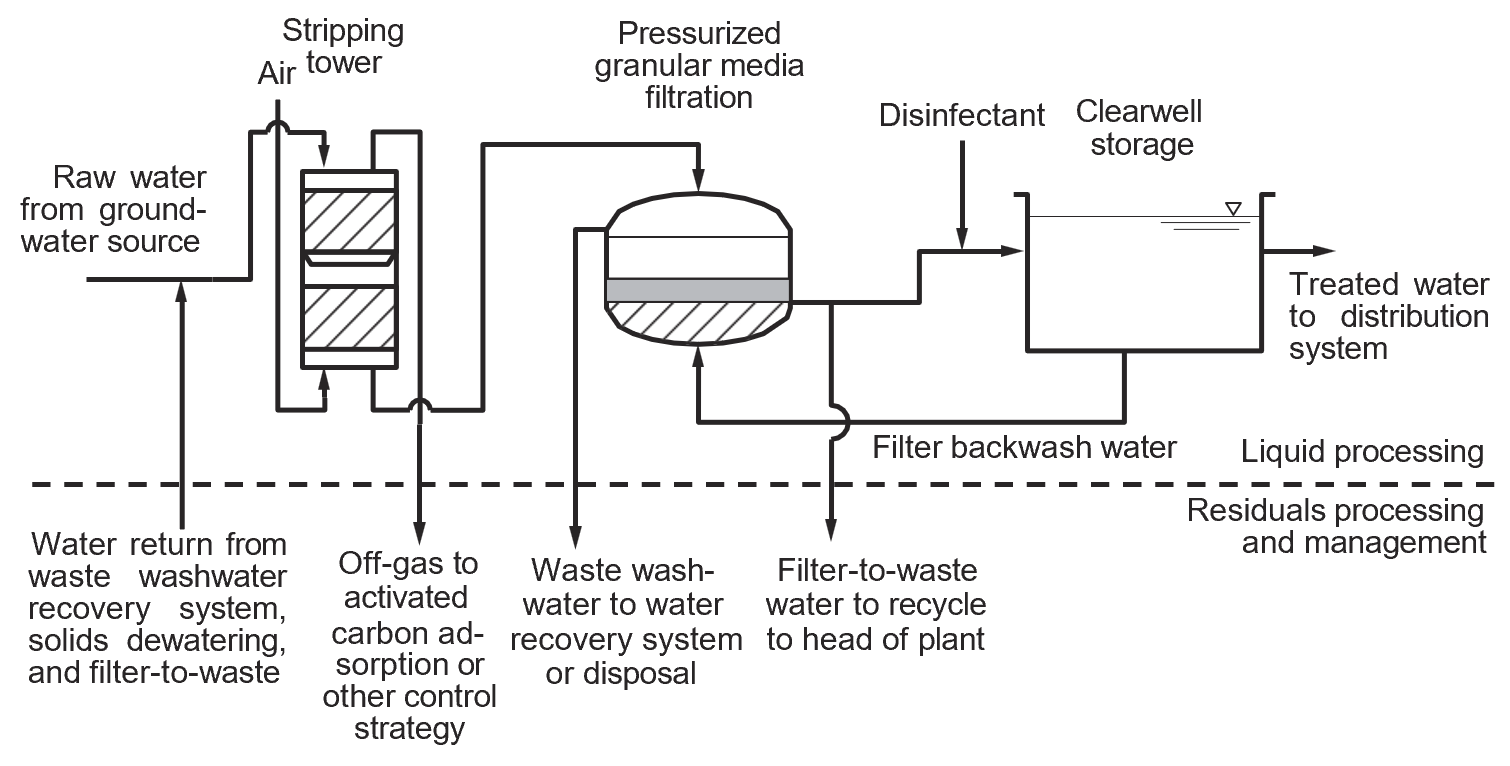
\includegraphics[scale=0.8]{GasVOCRemoval}\\
%\captionof{figure}{GasVOCRemoval 0.8}%\caption{}
%\end{center}
%\end{figure}
%
%\begin{figure}[H]
%\begin{center}
%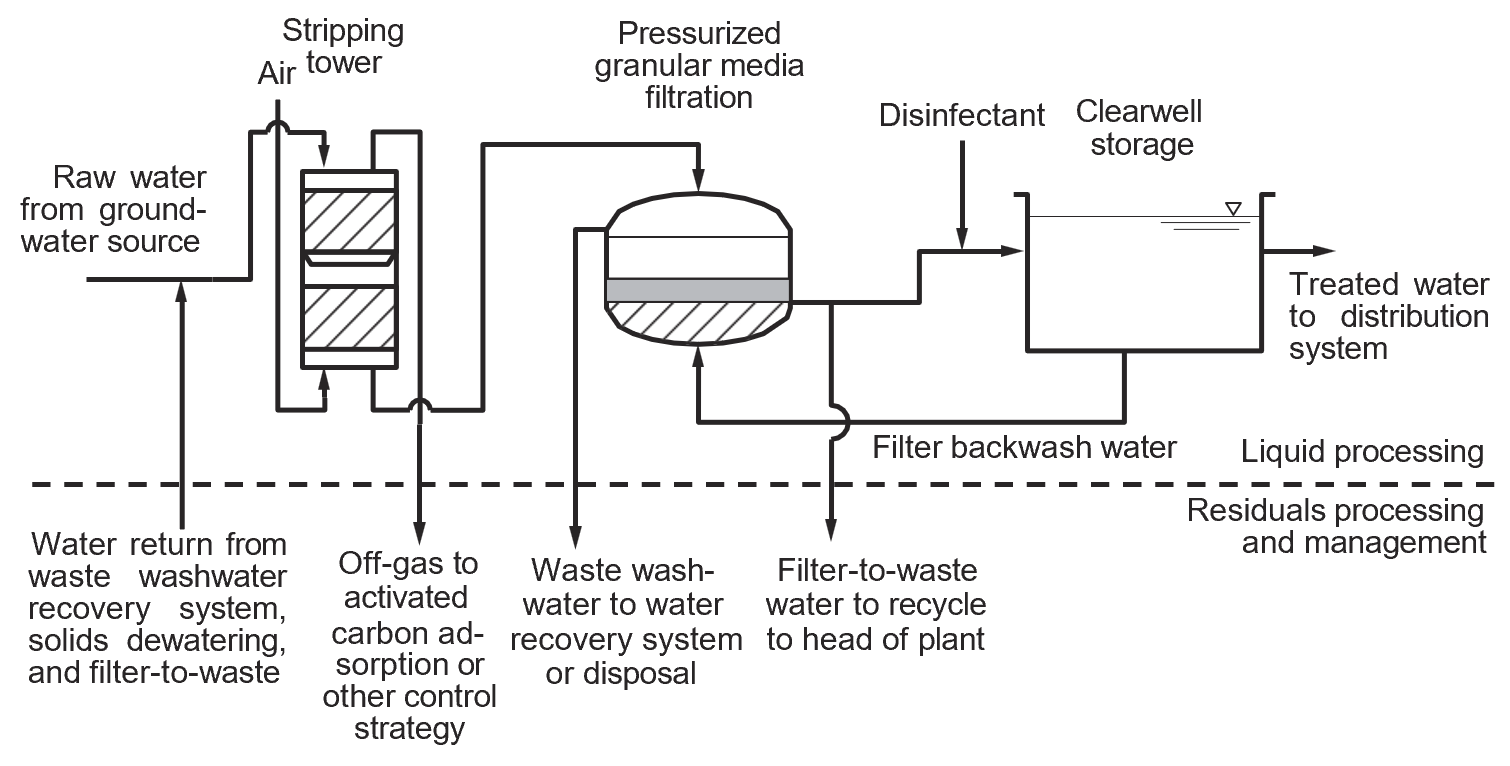
\includegraphics[scale=0.8]{GasVOCRemoval}\\
%\captionof{figure}{GasVOCRemoval 0.8}%\caption{}
%\end{center}
%\end{figure}
%
%
%
%
%

\subsubsection{Operation}\index{Operation}
\begin{itemize}
\item The removal mechanism in filtration involves straining – trapping larger particles and through adsorbtion where particles attach themselves to the filter media
\item Typical Filtration Rates:
\begin{itemize}
\item Slow Sand: 0.05 gpm/ft$^2$ - 3 feet sand
\item Rapid Sand: 2 gpm/ft$^2$ – 3 feet sand
\item Pressure filters: 3 gpm/ft$^2$
\item High Rate: 2-6 gpm/ft$^2$ – various media configurations
\end{itemize}

\item After a period of operation – filter cycle, the filter headloss increases because of the accumulation of the trapped solids.
\item Rapid filters are cleaned by backwashing using an upward, high-rate flow of water

\item Coagulation-flocculation is not required for cake filtration whereas chemical treatment is required for depth filtration.
\item Backwashing involves reversing the flow of water through the filter causing water to travel from the bottom of the filter to the top. 
\item Backwash is done at specific rates in order to most effectively remove the particulate material.  Backwashing process can be augmented by introducing low pressure air into the backwash line.
\item Backwash rates of 12-15 gpm/ft$^2$ or higher are common for sand, and rates for anthracite may range from 8 to 12 gpm/ft$^2$.
\item Wastewater used for the backwash is collected and removed from the filter. 






\item \textbf{Operational Problems}

Two common issues include:

\begin{itemize}

 

%black, blue, brown, cyan, darkgray, gray, green, lightgray, lime, magenta, olive, orange, pink, purple, red, teal, violet, white, yellow.

%\colorbox{declared-color}{text}

%\begin{tcolorbox}[width=\textwidth,colback={red},title={With true corners},outer arc=0mm,colupper=white]   

%   Air binding – vacuum generated due to higher water outflow than inflow causes violent upheaval impacting the media bed, gravel and/or underdrain.

    %\includegraphics[scale=0.5]{frogimage.png}

%\end{tcolorbox}   

\item \textbf{Air Binding} – vacuum generated due to higher water outflow than inflow causes violent upheaval impacting the media bed, gravel and/or underdrain.

 

\item \textbf{Mud balls} – these are formed as a result of inadequate backwashing and can cause the the filter to completely clog-up.

\end{itemize}
\end{itemize}

%\subsubsection{Greensand Filtration}\index{Greensand Filtration}
%\begin{itemize}
%\item 
%\end{itemize}
%\end{itemize}
%\subsubsection{Granulated activated carbon filter}\index{Granulated activated carbon filter}
%\begin{itemize}
%\item Granulated activated carbon filter\\
%\vspace{0.3cm}
%\begin{minipage}{.6\textwidth}
%\begin{itemize}
%\item Granulated Activated Carbon (\textbf{GAC}) filters have a layer of activated carbon on top of anthracite or sand.
%\item Activated carbon adsorbs various contaminants, such as tastes and odor-causing organics, THMs, and synthetic organics. 
%\item GAC is lighter than sand or anthracite and has an effective size of 0.55 to 0.65 mm. \item These filters have the problem of losing some carbon during the backwashing; therefore backwashing is properly controlled to prevent the excessive loss of GAC. 
%\item Commonly, backwashing causes 1 to 6 percent GAC loss per year.
%\item Solids carbon blocks when used in lieu of granular carbon are effective in Cryptosporidium and Giardia removal.
%\end{itemize}
%\end{minipage}
% \begin{minipage}{0.5\textwidth}
%        \centering
%       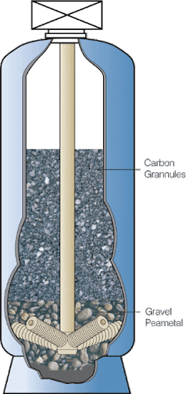
\includegraphics[scale=0.7]{GAC}
%    \end{minipage}\\
%
%\end{itemize}.

\section{Other treatment processes}
\subsection{Pre-chlorination}\index{Pre-chlorination}
\begin{itemize}
\item Pre-chlorination - chlorine is added to the incoming flow or, instead, added right before filtration.  Benefits of prechlorination include:
\begin{itemize}
\item Elimination of algae and other forms of aquatic life from the water so they won’t cause problems in the later stages of water treatment. 
\item Removal of tastes and odors
\item Control of biological growth throughout the water treatment system, thus preventing growth in the sedimentation tanks (where solids are removed from the water by gravity settling) and the filtration media (the filters through which the water passes after sitting in the sedimentation tanks). 
\item Oxidation of iron, manganese and/or hydrogen sulfide present in the water into a precipitate which can be removed in the sedimentation and filtration steps.
\end{itemize}
\end{itemize}

\subsection{Packed tower air stripping}\index{Packed tower air stripping}
\begin{itemize}
\item Water is sprayed on the top of a packed bed while air is blown at the bottom.
\item The packing provide the interface for the transfer of the contaminants from water into the air phase.
\item Air stripping is for removing:
\begin{itemize}
\item Volatile solids compounds
\item Carbon dioxide
\item Hydrogen sulfide
\item Ammonia
\end{itemize}
\end{itemize}
\begin{figure}[H]
\begin{center}
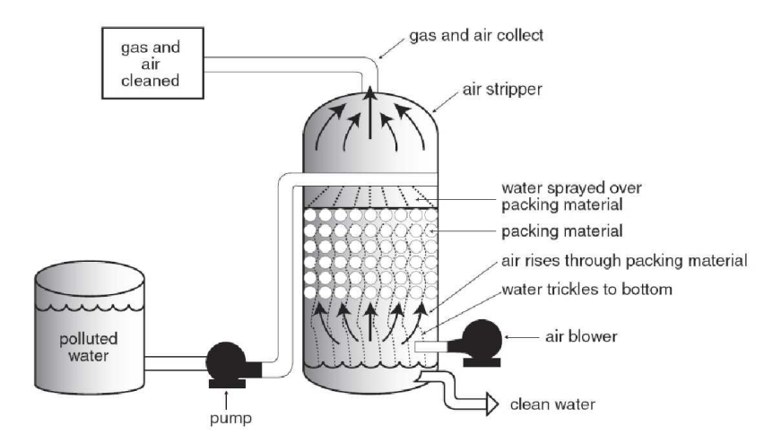
\includegraphics[scale=0.65]{AirStripping}\\
\captionof{figure}{Air stripper}%\caption{}\\
\end{center}
\end{figure}

\subsection{Aeration}\index{Aeration}
\begin{itemize}
\item In the aeration process the water is either pumped up into the air or allowed to fall over an aeration device

\item Aeration as a water treatment practice is used for the following operations:
\begin{itemize}
\item carbon dioxide reduction (decarbonation)
\item oxidation of iron and manganese found in many well waters (oxidation tower).  During aeration, iron and manganese get oxidized into an insoluble precipitate which is removed during filtration.
\item ammonia and hydrogen sulfide reduction (stripping)
\item Aeration is also an effective method of bacteria control.
\end{itemize}
\item Two general methods may be used for the aeration of water:
\begin{itemize}
\item Water-fall aeration Many variations of the water-fall principle are used for this type of aeration. The simplest configuration employs a vertical riser that discharges water by free fall into a basin.
\item Air diffusion aeration where air is diffused into a receiving vessel containing counter-current flowing water, creating very small air bubbles. This ensures good air-water contact for "scrubbing" of undesirable gases from the water.
\end{itemize}
\end{itemize}


\subsection{Iron and manganese sequestration}\index{Iron and manganese sequestration}
\begin{itemize}
\item Polyphosphates are used for sequestering iron and magnesium. Sequestration is the addition of chemicals to groundwater aimed at controlling problems caused by iron and manganese without removing them.
\item These chemicals are added to groundwater at the well head or at the pump intake before the water has a chance to come in contact with air or chlorine. This ensures that the iron and manganese stays in a soluble form.
\item If the water contains less than 1.0 mg/L iron and less than 0.3 mg/L manganese, using polyphosphates followed by chlorination can be an effective and inexpensive method for mitigating iron and manganese problems. 
\item No sludge is generated in this method. Below these concentrations, the polyphosphates combine with the iron and manganese preventing them from being oxidized. 
\item Any of the three polyphosphates (pyrophosphate, tripolyphosphate, or metaphosphate) can be used.
\item Applying sodium silicate and chlorine simultaneously has also been used to sequester iron and manganese. However, while this technique is reliable in the case of iron treatment, it has not been found to be effective in manganese control.  
\end{itemize}

\subsection{Fluoridation and defluoridation}\index{Fluoridation and defluoridation}
Fluoridation is the use of fluoride in the drinking water. Fluoride is an important component of bones and teeth. Fluoride deficiency causes weaker bones and tooth decay. Too much fluoride causes skeletal and dental fluorosis, resulting in brittle bones and mottled teeth, respectively.  An effective daily dose of fluoride is 0.9 to 1.7 mg/L. A dose less than 0.7 mg/L does not do the job, and more than 4.0 mg/L can cause fluorosis leading to irreversible demineralization of bone and tooth tissues.\\

The U.S. Department of Health and Human Services Agency (HHS) is recommending that water systems practicing fluoridation adjust their fluoride content to 0.7 mg/L, as opposed to the previous temperature-dependent optimal levels ranging from 0.7 mg/L to 1.2 mg/L.\\

EPA has set the maximum contaminant level for fluoride in the drinking water at 4mg/L \index{Fluoride!MCL}. Additionally, a secondary standard of 2.0 mg/L \index{Fluoride!SMCL} is intended as a guideline for an upper boundary level in areas which have high levels of naturally occurring fluoride.\\

Theoretically, any compound that forms fluoride ions in water solution can be used for increasing the fluoride content of a water supply. Most commonly used chemicals for this purpose include:\\
\begin{itemize}
\item Fluorosilicic acid fluorosilicic acid, as hexafluorosilicic acid (H$_2$SiF$_6$) which is a water-based solution used by most water systems in the United States. Fluorosilicic acid is also referred to as hydrofluorosilicate, FSA, or HFS.
\item Sodium fluorosilicate as disodium hexafluorosilicate (Na$_2$SiF$_6$) which is a dry salt additive, dissolved into a solution before being added to water, and
\item Sodium fluoride, a dry salt additive, typically used in small water systems, dissolved into a solution before being added to water.
\end{itemize}



In certain areas that have a naturally high level of fluoride in the groundwater defluoridation may have to occur.  Defluoridation methods include:
\begin{itemize}
\item Precipitation method utilizes chemical such as aluminum salts (i.e. alum) and lime.
\item  Ion-Exchange Methods utilizes different ion-exchange materials studied include bone, bone char and anion and cation exchange resins.
\item  Adsorption method uses chemical and physical adosrbents including activated carbon and alumina (Al$_2$O$_3$).  Activated alumina is used to treat water with fluoride concentrations from 4-20 mg/L in an adsorption process.
\end{itemize}

\subsubsection{Fluoride Dosing Chemicals Safety}
\begin{itemize}
\item Rubber gloves, coveralls, and protective eyewear should be worn when handling fluoride. 
\item Solid forms of fluoride are the most problematic to operators, since inhaling fluoride dust is very dangerous.  A dust collector should be used and a respirator should be worn when handling fluoride powders. 
\item Liquid forms, such as hydrofluosilicic acid, can also be dangerous.  Hydrofluosilicic acid produces poisonous fumes which must be vented and which are irritating to the skin.  The liquid itself can cause burns when allowed to touch skin.
\item The most extreme safety problem when dealing with fluoride is fluoride poisoning, which can be fatal.  However, fluoride poisoning occurs only when a large amount of fluoride - approximately one tablespoon - is ingested.  This is an amount much larger than would normally be inhaled while handling dry fluorides.  \item Accidental ingestion of fluoride chemicals can occur through contaminated food and drink.  The operator should always wash his hands after handling fluoride chemicals and should not eat, drink, or smoke in areas where fluorides are used or stored.\\
\end{itemize}

\subsection{Hardness removal}\index{Hardness removal}
\begin{itemize}
\item In almost every raw water supply, hardness is present as calcium and magnesium bicarbonate - (Ca/Mg)HCO$_3$, often referred to as carbonate hardness or temporary hardness. These compounds result from the action of acidic, carbon dioxide laden rain water on naturally occurring minerals in the earth, such as limestone.

CO$_2$ + H$_2$O = H$_2$CO$_3$\\

H$_2$CO$_3$ + CaCO$_3^-$ = Ca(HCO$_3$)$_2$

\item Hardness may also be present as a sulfate or chloride salt, referred to as noncarbonate or permanent hardness. These salts are caused by mineral acids present in rain water or the solution of naturally occurring acidic minerals.

\item Softening removes hardness and alkalinity making the product water more corrosive.  
\item It may be necessary to add corrosion-inhibiting materials to the finished water to protect the distribution system and prevent possible simultaneous compliance issues with other regulations like the Lead and Copper Rule.
\item Another option is to bypass a portion of water around the softening process and blending the treated and untreated waters are blended to produce an effluent with a total hardness around 50 to 75 mg/L as CaCO$_3$. 

\item Two common methods used to reduce hardness:
\begin{enumerate}
\item Cation exchange:
\begin{itemize}
\item In this process the calcium (Ca$^{+2}$) and magnesium (Mg$^{+2}$) ions that cause water hardness are replaced or exchanged with with a non-hardness ion like sodium. 
\item The exchange medium can be natural “zeolites” or synthetic resin beads that resemble wet sand and hold loosley the sodium ions provided by dissolving sodium chloride salt.
\item As hard water passes through a softener, the calcium and magnesium trade places with sodium ions. 
\item Eventually when the exchange medium becomes coated with calcium and magnesium ions, it must be recharged or regenerated.
\end{itemize}
\item Precipitation Softening
\begin{itemize}
\item Here the water is treated with lime or a combination of lime and soda ash (sodium carbonate, Na$_2$CO$_3$). 
\item These chemicals react with the hardness and natural alkalinity in the water to form insoluble compounds (precipitate) which are removed from the water by sedimentation and, usually, filtration.
\item Waters with moderate to high hardness and alkalinity concentrations (150-500 ppm as CaCO$_3$) are often treated in this fashion.
\begin{itemize}
\item Lime removes bicarbonates - which cause carbonate hardness. 
\item Soda ash is used to remove chemicals that cause non-carbonate hardness.
\end{itemize}
\item The addition of lime as either hydrated lime (calcium hydroxide - Ca(OH)$_2$) or as quicklime (CaO) results in:
\begin{itemize}
\item Increases the pH of water
\item Reaction with calcium bicarbonate Ca(HCO$_3$)$^-$ typically the major source of hardness converting it to CaCO$_3$.  For each molecule of calcium bicarbonate hardness removed, one molecule of lime is used. 
\item As the pH increases further, additional Ca(OH)$_2$ will then react with magnesium bicarbonate Mg(HCO$_3$) ultimately converting it to magnesium hydroxide (Mg(OH)$_2$.  For each molecule of magnesium bicarbonate hardness removed, two molecules of lime are used.
\item Calcium is removed in the 9.0-9.5 pH range and the pH needs to be at least 10.6 to remove magnesium.
\item Both CaCO$_3$ and Mg(OH)$_2$ have limited solubility in water and precipitate out.
\item Because CaCO$_3$ and Mg(OH)$_2$ precipitates are very slightly soluble, some hardness remains in the water--usually about 50 to 85 mg/l (as CaCO$_3$). This hardness level is desirable to prevent corrosion problems associated with water being too soft and having little or no hardness.
\end{itemize}
\item Use of lime along with soda ash  with results in:
\begin{itemize}
\item The magnesium non-carbonate hardness such as Mg(SO$_4$) is converted by lime to Mg(OH)$_2$ and Ca(SO$_4$) - a form of calcium non-carbonate hardness 
\item The calcium non-carbonate hardness - CaSO$_4$ is converted by soda ash to CaCO$_3$.  
\item For each molecule of non-carbonate calcium hardness removed, one molecule of soda ash is used.
\item For each molecule of non-carbonate magnesium hardness removed one molecule of lime plus one molecule of soda ash is used.
\item When water has minimal magnesium hardness, only calcium needs to be removed. Only enough lime and soda ash are added to water to raise pH to between 10.3 and 10.6, and calcium hardness will be removed from the water (but minimal magnesium hardness will be removed).
\item Extra lime addition is required to raise the pH above 10.6 to precipitate Mg(OH)$_2$ out of the water.
\item To improve magnesium reduction, which also improves silica reduction, sodium aluminate is added.  The sodium aluminate provides hydroxyl ion (OH$^-$) needed for improved magnesium reduction, without increasing calcium hardness in the treated water.  Additonal benefits of adding sodium aluminate comes from its formation of aluminum hydroxide which aids floc formation, conditions sludge blanket and helps reduce silica.
\end{itemize}
\item The portion of raw water may be bypassed 
\item Precipitation softening is often done in conjunction with coagulation and flocculation.
\item The precipitate formed is separated in the sedimentation tank as sludge.
\item The high pH, softened water produced is corrosive and \textbf{Recarbonation} \index{Recarbonation} of the softened water using carbon dioxide (CO$_2$) is conducted to lower the pH and thus its corrosivity.  
\item Lime softening produces large quantity of sludge.
\item \textbf{The reaction of quicklime with water leading to the formation of Ca(OH)$_2$ releases large quantity of heat and is dangerous if left uncontrolled.  Also, quicklime should never be stored with alum as the water of hydration in alum will react with quicklime causing an explosion}
\end{itemize}
\end{enumerate}
\end{itemize}

\begin{figure}[]
\begin{center}
\includegraphics[scale=0.48]{PrecipitationSOftening}\\
\captionof{figure}{Precipitation Softening}%\caption{}\\
\label{Precipitation softening}
\end{center}
\end{figure}

\subsection{Corrosion control}\index{Corrosion control}
\begin{itemize}
\item Corrosion is the gradual deterioration or destruction of metal surfaces by chemical and electrochemical processes.
\item As corrosive water stands or seals in pipes or tanks, it leaches metals from the piping, tanks, well casing, or other metal surfaces that water is in contact.
\item Corrosion can happen both from the inside of pipes and fittings and from the outside - because of the action of the external environment - including soils.
\item Lead and copper in service lines and household plumbing leach into the drinking water because of the corrosivity of water. 
\item Lead is a toxic metal that can be harmful to human health even at low exposure levels. Lead is persistent and can bioaccumulate in the body over time. 
\item The corrosivity of water will depend on the material of construction of the distribution system components and characteristics of water - water is less corrosive at higher pH and alkalinity.
\item Corrosion potential of the water on the distribution system components can be mitigated by chemical treatment:
\begin{itemize}
\item Adding alkalinity in the form of lime, soda ash, or caustic soda to make the water stable or slightly scale-forming. 
\item Orthophosphates are added to chemically react with lead and copper atoms forming lead and copper phosphate. The lead and copper phosphate is then electrochemically drawn back down onto the piping surface, where it forms a tough, water-resistant coating on the piping. 
\item Silicate compounds added to water also inhibit corrosion by forming a thin protective films on pipe walls.
\end{itemize}
\end{itemize}
\begin{table}[htp]
\captionsetup{justification=centering}
\scriptsize
\begin{tabular}{|p {2cm}|p {5cm}|p {7cm}|}
\hline
Treatment Method                               & How It Works                                                                                                                                                                                                                                             & What It Removes                                                                                                                                                                                                                                                                                                                                                                                                                                                    \\ \hline
Activated carbon filtration & As water flows through the filter contaminants   adsorb, or stick to, the surface of activated carbon particles.                                                                                                                        & Pesticides; organic compounds such as benzene and   carbon tetrachlo- ride; many odors; bacterial or colloidal iron or tannins when combined with continuous chlorination; radon; lead or copper if equipped   with special media; some other heavy metals in certain cases; chlorine;   chloramines; trihalomethanes. Filters with molded activated carbon blocks will treat Cryptosporidium and Giardia.
 \\ \hline

Reverse osmosis (RO)          &Contaminants are removed by forcing water through a   membrane which has microscopic holes. Water molecules pass through the   membrane but larger particles cannot. The membrane is flushed to remove   trapped contaminants.        & Certain tastes; some pesticides; high chloride content;   fluoride; nitrate; lead, copper, and other heavy metals; arsenic; Cryp tosporidium; viruses.                                                                                                                                                                                                                                                       \\
                                               &                                                                                                                                                                                                                                                          &                                                                                                                                                                                                                                                                                                                                                                                                                                                                    \\ \hline
Ion exchange water softening                   & As water passes through a resin   bed in the softener, calcium and magnesium in the water are exchanged for   sodium or potassium which do not create the nuisance problems associated with   hard water.                                                & Hard water (calcium and   magnesium); dissolved iron; manganese; will treat cadmium, copper and zinc if   operated properly.                                                                                                                                                                                                                                                                                                                                       \\ \hline


Sediment filtration                            & As water passes through a filter   made of sand, filter paper, compressed glass wool or other straining material   suspended particles such as sand, soil or other particles are trapped on   the filter.                                              & Sediment; acidic water when   preceded by soda ash feed; dissolved iron or manganese when preceded by   continuous chlorination, ozonation or aeration; turbidity.                                                                                                                                                                                                                                                                                             \\ \hline


Distillation & Water is heated to create steam which is then condensed to be collected   as treated water. Contaminants removed remain in the heating chamber or boil   off into the atmosphere. & Sediment; high salt content; high total dissolved solids; pesticides if   properly equipped with gas vent; fluoride; nitrate; lead, copper and other   heavy metals; arsenic; bacteria. 
\\ \hline

Aeration                                       & Oxygen is introduced into the water by an aerator. This oxidizes contaminants such as iron and manganese,   causing them to form solids which can then be filtered out of the water.   & Dissolved iron or manganese when followed by sediment filtration; may help reduce rotten egg odor from   dissolved hydrogen sulfide gas; radon.                                                                                                                                                                                                                                                                                                                  \\ \hline

De-Aeration                & Mix air with water to remove dissolved gases from the water. Aeration and                                                                                                                                                                              &Dissolved   hydrogen sulfide gas; radon. De-aeration equipment sometimes are very similar, but are designed for different   treatment goals.                                                                                                                                                   
\\ \hline

Continuous Chlorination       & Chlorine is fed or injected into the water to   kill bacteria and other microbial contaminants, as well as to oxidize iron   and manganese causing them to form solids which can then be filtered out.                             & Dissolved iron or manganese when   followed by sediment filtration; rotten egg odor from dissolved hydrogen   sulfide gas or sulfate-reducing bacteria (followed by activated carbon                                                                                                                                                                                                                                                                              filtration);   bacterial or colloidal iron or tannins when combined with activated carbon   filtration; bacteria; Giardia; viruses.                                                                                                                                                                                                                                                                                                                                \\ \hline 

Ultraviolet (UV) radiation    &As water passes through the system, a special lamp produces ultraviolet   light that kills bacteria and other microbial contaminants.
                                               &                                                                                                                                                                                                                                                          \\ \hline

Ozonation                     & Water enters a system where ozone is produced and mixed with the water,   a chemical form of pure oxygen,                                                                                                                                                                                     & Bacteria; Giardia; Cryptosporidium; viruses;   Ozonation destroys bacteria and other   microbial pathogens and oxidizes compounds such as iron and manganese causing   them to form solids which can then be filtered out using sediment filtration.
\\ \hline

Ultra,   micro, and nano filtration            & As water passes through a   filter, suspended particles are trapped on the filter. Particles removed   depends upon the size of the pores in the filter. Pore sizes from smallest to   largest are nanofiltration, ultra filtration and microfiltration. & Cryptosporidium; Giardia; viruses.                                                                                                                                                                                                                                                                                                                                                                                                                                 \\ \hline
\end{tabular}
\caption{Summary of water treatment methods} \index{Treatment!Summary of water treatment methods}
\label{Summary of water treatment methods}
\end{table}

\section{Best Available Technology (BAT)} \index{Best Available Technology (BAT)}

Below is the summary of BATs - the very best (state-of-the-art) control and treatment measures that have been developed, or are capable of being developed, and that are economically achievable, identified in the California Code of Regulations. 

\subsection{BATs for inorganics} \index{Best Available Technology (BAT)!Inorganics} 

% Please add the following required packages to your document preamble:
% \usepackage[normalem]{ulem}
% \useunder{\uline}{\ul}{}
\begin{table}[H]
\begin{tabular}{|l|l|}
\hline
\multicolumn{1}{|c|}{\textbf{Chemical}} & \multicolumn{1}{c|}{\textbf{Best Available Technologies (BATs)}} \\ \hline
Aluminum                                & 10                                                               \\ \hline
Antimony                                & 2, 7                                                             \\ \hline
Arsenic                                 & 1, 2, 5, 6, 7, 9, 13                                             \\ \hline
Asbestos                                & 2, 3, 8                                                          \\ \hline
Barium                                  & 5, 6, 7, 9                                                       \\ \hline
Beryllium                               & 1, 2, 5, 6, 7                                                    \\ \hline
Cadmium                                 & 2, 5, 6, 7                                                       \\ \hline
Chromium                                & 2, 5, 6$^a$ , 7                                                    \\ \hline
Cyanide                                 & 5, 7, 11                                                         \\ \hline
Fluoride                                & 1                                                                \\ \hline
Mercury                                 & 2 b , 4, 6 $^b$ , 7 b                                               \\ \hline
Nickel                                  & 5, 6, 7                                                          \\ \hline
Nitrate                                 & 5, 7, 9                                                          \\ \hline
Nitrite                                 & 5, 7                                                             \\ \hline
Perchlorate                             & 5, 12                                                            \\ \hline
Selenium                                & 1, 2 $^c$ , 6, 7, 9                                                 \\ \hline
Thallium                                & 1, 5                                                             \\ \hline
\end{tabular}
\end{table}
$^a$ BAT for chromium III (trivalent chromium) only.\\
$^b$ BAT only if influent mercury concentrations <10 $\mu$g/L.\\
$^c$ BAT for selenium IV only.\\

where:\\
1 = Activated Alumina\\
2 = Coagulation/Filtration (not BAT for systems <500 service connections)\\
3 = Direct and Diatomite Filtration\\
4 = Granular Activated Carbon\\
5 = Ion Exchange\\
6 = Lime Softening (not BAT for systems <500 service connections)\\
7 = Reverse Osmosis\\
8 = Corrosion Control\\
9 = Electrodialysis\\
10 = Optimizing treatment and reducing aluminum added\\
11 = Chlorine oxidation\\
12 = Biological fluidized bed reactor\\
13 = Oxidation/Filtration\\

\subsection{BATs for microbiological contaminants} \index{Best Available Technology (BAT)!Microbiological contaminants} 
Best available technology (BAT) (for a public water system serving more than 10,000 persons), affordable technology (for a public water system serving 10,000 or fewer persons), treatment techniques, or other means available for achieving compliance with the E. coli MCL are as follows:\\
(a) Protection of wells from fecal coliform contamination by appropriate placement and construction;\\
(b) Maintenance of a disinfectant residual throughout the distribution system;\\
(c) Proper maintenance of the distribution system including appropriate pipe replacement and repair procedures, main flushing programs, proper operation and maintenance of storage tanks and reservoirs, cross connection control, and continual maintenance of positive water pressure in all parts of the distribution system;\\
(d) Filtration and/or disinfection of approved surface water, in compliance with Section 64650, or disinfection of groundwater, in compliance with Section 64430, using strong oxidants such as chlorine, chlorine dioxide, or ozone; and\\
(e) For a system using groundwater, compliance with the groundwater portion of a Drinking Water Source Assessment and Protection Program.


\subsection{BATs for radionuclides} \index{Best Available Technology (BAT)!Radionuclides} 
% Please add the following required packages to your document preamble:
% \usepackage[table,xcdraw]{xcolor}
% If you use beamer only pass "xcolor=table" option, i.e. \documentclass[xcolor=table]{beamer}
% \usepackage[normalem]{ulem}
% \useunder{\uline}{\ul}{}
\begin{table}[H]
\begin{tabular}{|l|p{8cm}|}
\hline
\textit{Radionuclide} & \textit{Best Available Technology} \\ \hline
Combined radium-226 and radium-228                                       & Ion exchange, reverse osmosis, lime softening                                        \\ \hline
Uranium                                                                   & Ion exchange, reverse osmosis, lime softening, coagulation/filtration                 \\ \hline
Gross alpha particle activity                                             & Reverse osmosis                                                                      \\ \hline
Beta particle and photon radioactivity                                    & Ion exchange, reverse osmosis                                                     \\ \hline
\end{tabular}
\end{table}

\section{Chemical feed systems} \index{Chemical feed systems}
\begin{itemize}
\item Chemical feed systems are designed for automated and precise injection (dosing) of chemicals into the water to be treated. 
\item Chemical feed systems are mainly employed for the following types of water treatment:
\begin{itemize}
\item Disinfection
\item Flocculation and Coagulation
\item Nutrient Removal
\item Sludge Conditioning
\item Alkalinity Supplementation
\item Corrosion Inhibition
\end{itemize}
\item The chemical feed systems is comprised of different components and is typically designed to ensure suitability with the chemical dispensed and the environment.
\item There are three types of chemicals used by chemical feed systems: 
\begin{enumerate}
\item Dry Chemicals: These chemicals are in dry, powdered form. Sodium bicarbonate, calcium hypochlorite, calcium chloride, algaecides, and soda ash are a few popular types of dry chemicals. Dry chemicals may or may not be mixed with liquids.
\item Liquid Chemicals: These are most common form of chemicals used due to the ease of use. Aluminum sulfate or liquid alum, 50\% sodium hydroxide, and caustic soda are a few liquid chemicals used regularly.
\item Gaseous Chemicals: Chlorine gas is widely used in water treatment for disinfection.
\end{enumerate}
\end{itemize}

%\subsection{Key Components of a Chemical Feed System} \index{Chemical feed systems!Components}
\subsection {Types of chemical feed systems}\index{Chemical feed systems!Types}

\begin{itemize}
\item Chemicals are fed into the water stream in different ways based on the required feed rate and feed pump output. 
\item Typically, solid and liquid chemicals can be fed in any of the following ways:
\begin{itemize}
\item Continuous Feed: This system is commonly used for liquid chemicals, which are continuously fed into the water tank. This feed system is commonly employed for deposit control in once-through systems, as well as domestic water chlorination. The continuous feed may be provided by a gravity drip feed, where the feed rate is regulated by a needle valve.
\item Shot/slug Feed: The chemical is shot/slug-fed by an on-off control on a feeder pump. It may also be discharged from a measuring chamber or a calibrated pump. This type of feeding is widely used in bio-oxidation basins or cooling systems with high system volume to blowdown ratio.
\end{itemize}
\item For gaseous chemicals dosing, the following two methods are utilized.
\begin{itemize}
\item Solution Feed: This type of feeding is seen in vacuum-type feeders, where gas is drawn to the piping system by vacuum. If there is any leak in piping then it leads to vacuum loss, and as a result, the system is shut down for supply. The vacuum feeders use ejectors to create a vacuum required for operation.
\item Direct Feed: In this feed, gas is fed into the flow stream to be treated. This involves the direct injection of gas under high pressure. This type of feeding is usually restricted to small applications, which have no regular water supply for solution feed.
\end{itemize}
\end{itemize}

\subsection{Delivery systems}\index{Chemical feed systems!Components!Delivery}
\begin{itemize}
\item Feed pumps carry chemicals for dosing.   
\item \textbf{Metering pumps} are the most common types of feed pumps used for \textbf{liquid} chemical feed systems. Types of chemical metering pumps used in the water industry include:
\begin{itemize}
\item Diaphragm Pumps: 
\begin{itemize}
\item A diaphragm pump consists of one or more pumping chambers alternately filled and discharged by the movement of flexible diaphragms and check valves on the inlet and outlet.
\item The diaphragm pump is composed of the following:
\begin{itemize}
\item A chamber used to pump the fluid
\item A diaphragm or diaphragms operated by either electric or mechanical means
\item Two valve assemblies: a suction valve assembly and a discharge valve assembly
\end{itemize}
\begin{figure}[H]
\begin{center}
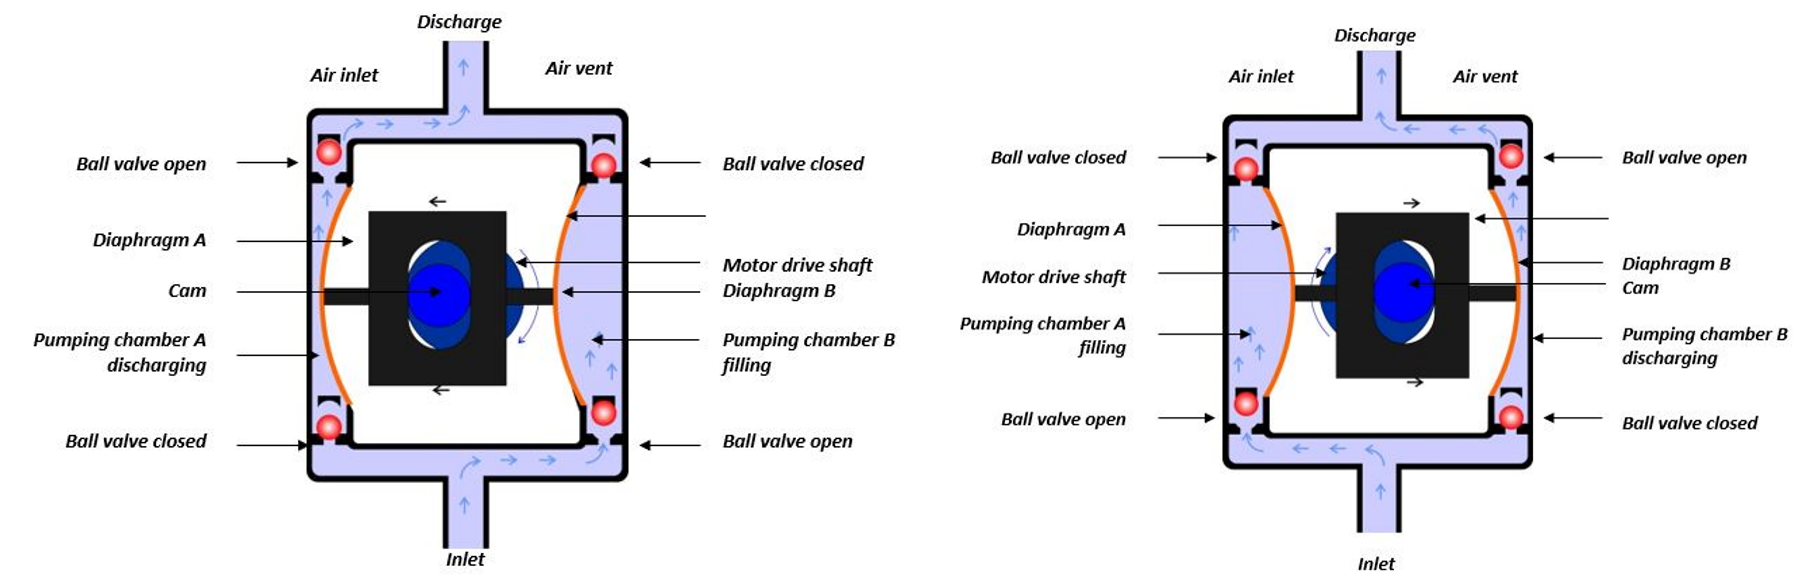
\includegraphics[scale=1]{AODDPump}
\vspace{0.2cm}
\caption{Air operated double diaphragm pump} \index{Pump type!Diaphragm pump}
\end{center}
\end{figure}
\item These pumps are widely used to handle mostly all liquid chemicals, as well as sludges and slurries with ease.
\end{itemize}
\item Peristaltic Pumps:
\begin{itemize}
\item These pumps are also known as roller pumps because it uses a set of rollers to pump the fluid. 
\item The chemical fluid to be pumped is contained in a flexible tube, which is positioned inside a pump casing.
\item The rotors equipped with rollers compress the tube, thereby forcing the fluid to move towards the pipe. The pump comes to its original position after the fluid moves out. This whole process is known as peristalsis. 
\item Peristaltic pumps are suited for applications requiring small feed rates of < 0.1 gallons per hour.
\end{itemize}
\begin{figure}[H]
\begin{center}
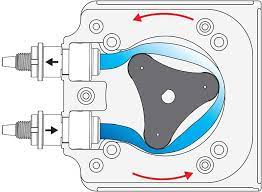
\includegraphics[scale=0.4]{PeristalticPump}\\
\caption{Peristaltic pump} \index{Pump type!Peristaltic pump}
\end{center}
\end{figure}
\item Other Metering pumps include: Packed Plunger Pumps, Liquid Gravity Feeders and Jet Pumps (Eductors)
\end{itemize}




\item For dry chemicals the following types of feeder systems are used:
\begin{itemize}
\item Volumetric Feeders: These feeders dispense an accurate amount of powdered material. Volumetric feeders are generally used for feeding dry chemicals such as lime slaking, lime feed, clay feed, dry polymer, and so on.
\item Gravimetric Feeders: The feeders feed chemicals by weight. Gravimetric feeders assure accuracy within 1-2\%.
\end{itemize}

\begin{figure}[H]
\begin{center}
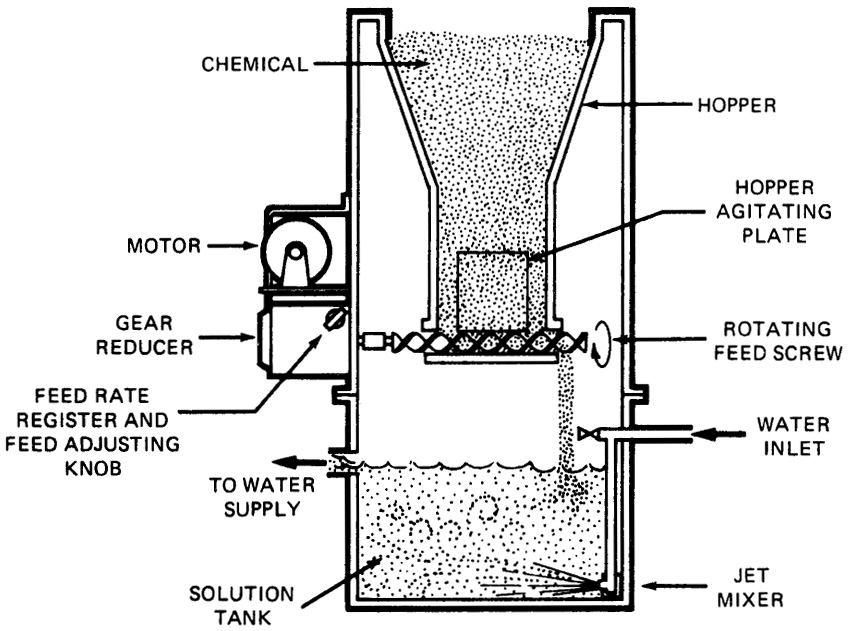
\includegraphics[scale=.6]{VolumetricChemicalFeeder} \hspace{0.7 cm}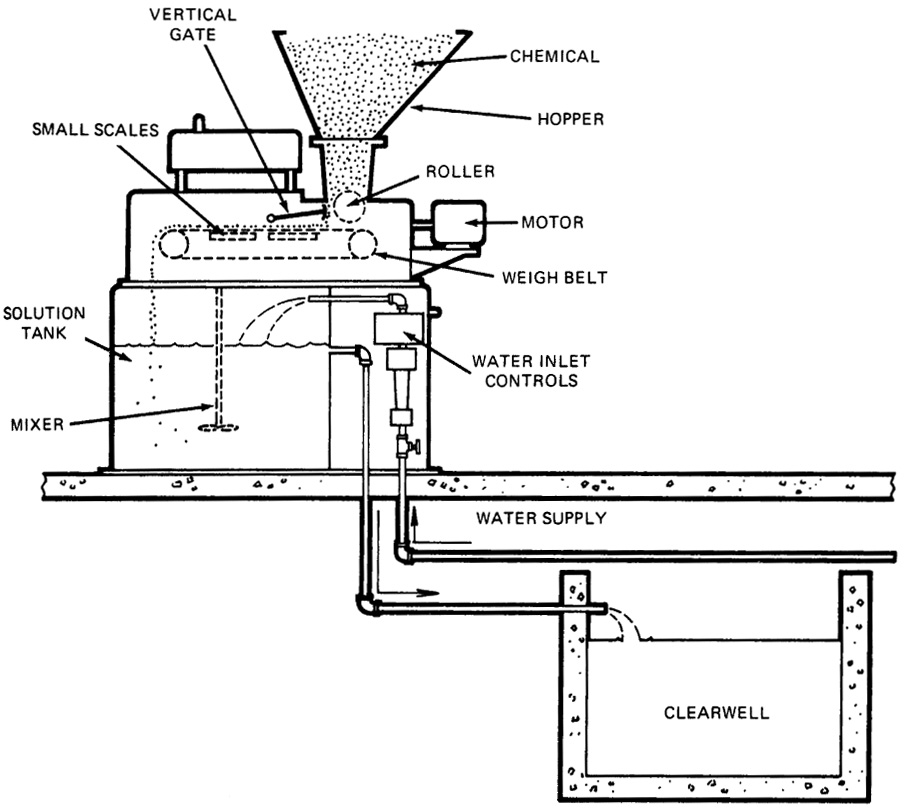
\includegraphics[scale=0.6]{GravimetricChemicalFeeder}\hspace{0.7 cm}\\
\vspace{0.2cm}
\hspace{1 cm}Volumetric Feeder\hspace{5 cm}Gravimetric Feeder\\
\caption{Dry chemical feeders}
\end{center}
\end{figure}


\item Gaseous chemicals are transferred using gas feeders. To ensure safety, particularly when used in an application involving chemical such as chlorine, these gas systems are used under vacuum. To use these systems, special equipment and arrangements need to be done. Self-contained breathing equipment, special containment chorine rooms, chlorine gas detectors, as well as chlorine air room scrubbers are some of the requirements.
\end{itemize}
\subsection {Chemical storage systems}\index{Chemical feed systems!Components!Storage}
Solution tanks are the chemical storage systems used for holding chemical solutions to be fed into the water. There are three types of chemical storage systems used:
\begin{itemize}
\item Bulk Storage: The storage tank of this type can hold liquid chemicals in bulk. The chemicals for treatment are delivered by a carrier or a vendor truck. The tank is usually positioned near the feed system.
\item Semi Bulk Storage: This type of storage is ideal for applications that do not use chemical feeds regularly. Semi bulk storage tanks are designed in such a way that the tanks can be stored easily by stacking above one another when not in use.
\item Drum Storage: This was one of the most popular methods of chemical storage until a few years back. Safe disposal of drums after the end of their lifespan was one of the key challenges faced by users. To avoid this, nowadays, reusable containers - totes are used.
\end{itemize}

\subsection{Accessories}\index{Chemical feed systems!Components!Accessories}

\begin{itemize}
\item Mixers: The job of the mixer is to rapidly disperse the chemical additives to ensure a uniform mixture.  A rapid (or flash) mixer utilizes specifically designed impeller to uniformly disperse and blend chemicals, such as coagulant aids, chlorine, and sulfur dioxide, into the process stream.  Flash mixer can be installed in a tank, process chamber or pipe.
\begin{figure}[H]
\begin{center}
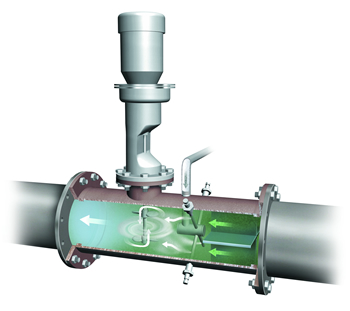
\includegraphics[scale=.4]{FlashMixer1} \hspace{3 cm}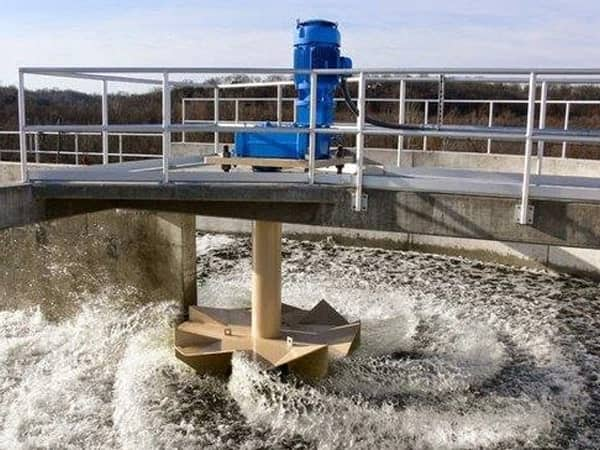
\includegraphics[scale=0.27]{FlashMixer2}\\
\vspace{0.2cm}
\hspace{1 cm}In-line Flash Mixer\hspace{4.5 cm}Process Flash Mixer
\caption{Flash mixers}
\end{center}
\end{figure}
\item Timers: Timers used to control the function of mixers, as well as the feeding of chemicals.
\item Alarms: Alarms are typically used as monitoring systems for different components of the chemical dosing system. They can be set to monitor tank levels, chemical feed rates, pump status, and changed operating conditions. Alarms help to reduce damages caused due to dry running or change in operating variables, or some unspecified conditions.
\item Level Gauges: As the name indicates, these devices are used to monitor the level of chemicals in tanks.
\item Control Panels: The control panel may also contain lights that indicate the status of the pumps, various alarm conditions, and hour meters.
\end{itemize}

\subsection {Chemical control systems}\index{Chemical feed systems!Control systems}
Typical types of chemical control systems include:
\begin{itemize}
\item Manual Controls: This is one of the simplest, yet popular controls employed in the water industry. The output of the pump is set manually using dials or knobs, and the pump is put on or off using a manual switch. Sometimes, the power supply on the pump is put on or off for operating or closing the pump.
\item Automatic chemical dosing control instrumentation is usually set up as either a “feed forward” or a “feedback” loop. 
\begin{itemize}
\item An example of a feed forward loop would be a venturi flow meter which is located forward of the chlorine feed point sending a signal to change a chlorine dosage based on a change in flow. 
\item An example of a feedback loop would be a chlorine analyzer located downstream of the chlorine dosage point, changing the chlorine dosage based on a change in residual downstream of the chlorinator.
\end{itemize}
\item On-off Constant Rate Mode: In this type of pump control, the pump on and off is automated. This control is more apt for cooling towers or other similar applications that do not require a continuous or regular feed of chemicals. In short, it is most suitable for controlling acid feed rates at low or high pH setpoints.
\end{itemize}

% \begin{tcolorbox}[breakable, enhanced,
% colframe=blue!25,
% colback=blue!10,
% coltitle=blue!20!black,  
% title= Chapter Assessment]
% \begin{enumerate}
% \item What is the recommended loading rate for copper sulfate for algae control at an alkalinity greater than 50 mg/L?
% \begin{enumerate}
% \item 0.9 lb of copper sulfate per acre of surface area
% \item 1.9 lb of copper sulfate per acre of surface area
% \item 2-4 lb of copper sulfate per acre of surface area
% \item.4 lb of copper sulfate per acre of surface area
% \end{enumerate}

% \item The basic goal for water treatment is to \rule{2cm}{0.3pt}.
% \begin{enumerate}
% \item Protect public health
% \item Make it clear
% \item Make it taste good
% \item Get stuff out
% \end{enumerate}

% \item Greensand can be operated in either \rule{2cm}{0.5pt} regeneration or \rule{2cm}{0.5pt} regeneration modes.
% \begin{enumerate}
% \item Continuous or intermittent
% \item Fast or slow
% \item Hot or cold
% \item Constant or unusual
% \end{enumerate}

% \item The two most common types of chlorine disinfection by-products include:
% \begin{enumerate}
% \item TTHM and HAA5
% \item TTHA of HMM5
% \item Turbidity and color
% \item Chloride and fluoride
% \end{enumerate}

% \item GAC contactors are used to reduce the amount of \rule{2cm}{0.5pt} contaminants in water.
% \begin{enumerate}
% \item Inorganic
% \item Turbidity
% \item Particle
% \item Organic
% \end{enumerate}

% \item List the five types of surface water filtration systems.
% \begin{enumerate}
% \item Bag filtration, cartridge filtration, fine filtration, coarse filtration, media filtration
% \item Conventional treatment, direct filtration, slow sand filtration, diatomaceous earth filtration, membrane filtration
% \item Turbidity filtration, color filtration, bag filtration, fine filtration, media filtration
% \item None of the above
% \end{enumerate}

% \item Describe two primary methods used to control taste and odor?
% \begin{enumerate}
% \item Oxidation and adsorption
% \item Filtration and sedimentation
% \item Mixing and coagulation
% \item Sedimentation and clarification
% \end{enumerate}

% \item The adsorption process is used to remove:
% \begin{enumerate}
% \item Organics or inorganics
% \item Bugs or salts
% \item Organisms or dirt
% \item Color or particles
% \end{enumerate}

% \item The solid that adsorbs a contaminant is called the:
% \begin{enumerate}
% \item Adsorbent
% \item Adsorbate
% \item Sorbet
% \item Rock
% \end{enumerate}

% \item What is a method of reducing hardness?
% \begin{enumerate}
% \item Softening
% \item Hardening
% \item Lightning
% \item Flashing
% \end{enumerate}


% \item Bag and cartridge filters are used to remove which two pathogenic microorganisms?
% \begin{enumerate}
% \item Viruses and giardia
% \item Giardia and cryptosporidium
% \item Viruses and bacteria
% \item None of the above
% \end{enumerate}

% \item The process of cleaning a filter by pumping water up through the filter media is called \rule{2cm}{0.3pt} the filter.
% \begin{enumerate}
% \item Backwashing
% \item Rewashing
% \item Purging
% \item Lifting
% \end{enumerate}

% \item In a typical water treatment plant, alum would be added into the \rule{2cm}{0.3pt} mixer.
% \begin{enumerate}
% \item Speed
% \item Large
% \item Slow
% \item Flash
% \end{enumerate}

% \item When comparing conventional treatment with direct filtration, what process unit is in the conventional treatment plant that is not in the direct filtration plant?
% \begin{enumerate}
% \item Filter
% \item Clarifier
% \item Mixer
% \item Detention
% \end{enumerate}

% \item List the basic processes, in the proper order, for a conventional treatment plant.
% \begin{enumerate}
% \item Coagulation, flocculation, sedimentation, filtration
% \item Flocculation, coagulation, sedimentation, filtration
% \item Filtration, coagulation, flocculation, sedimentation
% \item Coagulation, sedimentation, flocculation, filtration
% \end{enumerate}

% \item The four most common oxidants include:
% \begin{enumerate}
% \item Chlorine, potassium permanganate, ozone, chlorine dioxide
% \item Chlorides, soap, air, coagulants
% \item Air, chemicals, sodium, chloride
% \item Flocculants, coagulants, sediments, granules
% \end{enumerate}

% \item  When operating a filter, one of the operational concerns is the difference between the pressure or head on top of the filter and the pressure or head at the bottom of the filter. This difference is called \rule{2cm}{0.3pt} pressure.
% \begin{enumerate}
% \item Different
% \item Differential
% \item High
% \item Low
% \end{enumerate}

% \item  What type of polymer is used to improve the efficiency of the sedimentation
% process?
% \begin{enumerate}
% \item Cationic
% \item Nonionic
% \item Anionic
% \item All of the above
% \end{enumerate}

% \item A(n) \rule{2cm}{0.3pt} polymer is commonly used as a coagulant.
% \begin{enumerate}
% \item Anionic
% \item Cationic
% \item Nonionic
% \item Ionic
% \end{enumerate}


% \item A(n) \rule{2cm}{0.3pt} polymer is used to enhance flocculation.
% \begin{enumerate}
% \item Anionic
% \item Cationic
% \item Nonionic
% \item Ionic
% \end{enumerate}

% \item Al$_2$(SO$_4$)$_3$ • 18H$_2$O is the chemical formula for:
% \begin{enumerate}
% \item Alum
% \item Iron
% \item Manganese
% \item Lead
% \end{enumerate}

% \item Particles that are less than 1 $\mu$m in size and will not settle easily and are called:
% \begin{enumerate}
% \item Light particles
% \item Colloidal particles
% \item Colored particles
% \item Flat particles
% \end{enumerate}

% \item The sedimentation portion of water treatment is also called a(n):
% \begin{enumerate}
% \item Clarifier
% \item Filter
% \item Adsorber
% \item Water treater
% \end{enumerate}

% \item Slowly agitating coagulated materials is the process of:
% \begin{enumerate}
% \item Flocculation
% \item Coagulation
% \item Sedimentation
% \item Filtration
% \end{enumerate}

% \item The process of decreasing the stability of colloids in water is called:
% \begin{enumerate}
% \item Flocculation
% \item Coagulation
% \item Sedimentation
% \item Clarification
% \end{enumerate}

% \item The chemical oxidation process in water treatment is typically used to aid in the
% removal of :
% \begin{enumerate}
% \item Organic contaminants
% \item Inorganic contaminants
% \item Large contaminants
% \item None of the above
% \end{enumerate}

% \item Flocculation, sedimentation, filtration, and adsorption are \rule{2cm}{0.3pt}
% processes.
% \begin{enumerate}
% \item Physical
% \item Chemical
% \item Biological
% \item Mechanical
% \end{enumerate}

% \item Oxidation, coagulation, and disinfection are \rule{2cm}{0.3pt} processes.
% \begin{enumerate}
% \item Physical
% \item Chemical
% \item Biological
% \item Mechanical
% \end{enumerate}

% \item A precipitate can be formed after which one of the following processes:
% \begin{enumerate}
% \item Oxidation
% \item Flocculation
% \item Filtration
% \item Adsorption
% \end{enumerate}

% \item Water that is safe to drink is called \rule{1cm}{0.5pt}  water.
% \begin{enumerate}
% \item Potable
% \item Palatable
% \item Good
% \item Clear
% \end{enumerate}
% \end{enumerate}
% \end{tcolorbox}